\documentclass[12pt,a4paper]{article}

\usepackage[utf8]{inputenc}
\usepackage{mathtools}
\usepackage{amssymb}
\usepackage{ntheorem}
\usepackage[framemethod=TikZ]{mdframed}
\usepackage{amsmath}
\usepackage[hidelinks]{hyperref}
\usepackage{cleveref}
\usepackage{fancyhdr}
\usepackage{lastpage}
\usepackage{geometry}
\usepackage{arydshln}
\usepackage{url}
\usepackage{setspace}
\usepackage[T1]{fontenc}
\usepackage{mathptmx}
\usepackage{framed}
\usepackage{pifont}

\geometry{a4paper, left=2cm, right=2cm, bottom=2cm, top=2cm}

\pagestyle{fancy}
\fancyhead{}
\fancyhead[L]{\leftmark}
\fancyhead[R]{\rightmark}
\fancyfoot{}
\fancyfoot[C]{\thepage}
%\renewcommand{\headrulewidth}{0pt}
\renewcommand{\footrulewidth}{0pt}

\theorembodyfont{\upshape}
\theoremseparator{.}
\newtheorem{thm}{Theorem}[subsection]
\newtheorem{df}{Definition}[subsection]
\newtheorem{eg}{Example}[subsection]
\newenvironment*{sol}{\par\indent\textbf{\textit{Solution. }}\par}{\par\hfill{$\square$}\par}
\newtheorem*{rmk}{\indent Remark}
\newenvironment*{prf}{\par\indent\textbf{\textit{Proof. }}\par}{\par\hfill$\blacksquare$\par}
\newtheorem*{ext}{\indent Extension}

\linespread{1.25}

\title{Emory University\\\textbf{MATH 211 - Advanced Calculus (Multivariable) Learning Notes}}
\author{Jiuru Lyu}
\date{\today}

\linespread{1.22}

\def\Z{{\mathbb{Z}}}
\def\R{{\mathbb{R}}}
\def\C{{\mathbb{C}}}
\def\Q{{\mathbb{Q}}}
\def\E{{\mathbb{E}}}
\def\d{{\mathrm{d}}}
\def\i{{\mathrm{i}}}
\def\RE{{\mathrm{Re}}}
\def\IM{{\mathrm{Im}}}
\def\Arg{{\mathrm{Arg}}}
\def\cis{\mathrm{cis}}
\def\Proj{\mathrm{Proj}}
\def\qed{\rightline{$\blacksquare$}}
\def\ddx{\frac{\d}{\d x}}
\def\dydx{\frac{\d y}{\d x}}
\def\ddt{\frac{\d}{\d t}}
\def\dx{\d x}
\def\der{\partial}
\def\pdx{\der x}
\def\pdx{\der y}
\def\pdfdx{\frac{\der f}{\der x}}
\def\pdfdy{\frac{\der f}{\der y}}
\def\pdfdxdx{\frac{\der^2 f}{\der x\ \der x}}
\def\pdfdydy{\frac{\der^2 f}{\der y\ \der y}}
\def\pdfdxdy{\frac{\der^2 f}{\der x\ \der y}}
\def\pdfdydx{\frac{\der^2 f}{\der y\ \der x}}
\def\pddx{\frac{\der }{\der x}}
\def\pddy{\frac{\der }{\der y}}
\def\vecx{\vec{x}}
\def\vecy{\vec{y}}
\def\vecv{\vec{v}}
\def\vecw{\vec{w}}
\def\vecu{\vec{u}}
\def\veca{\vec{a}}
\def\vecb{\vec{b}}
\def\vecc{\vec{c}}
\def\vecd{\vec{d}}
\def\vecr{\vec{\boldsymbol{\textbf{r}}}}
\def\vecn{\vec{n}}
\def\vece{\boldsymbol{\textbf{e}}}
\def\veci{\hat{\boldsymbol{\textbf{i}}}}
\def\vecj{\hat{\boldsymbol{\textbf{j}}}}
\def\veck{\hat{\boldsymbol{\textbf{k}}}}
\def\DNE{\mathrm{D.N.E.}}
\def\LI{\mathrm{L.I.}}
\def\st{\mathrm{ s.t. }}

\begin{document}
\maketitle
\tableofcontents
\newpage

\section*{Preface}
These is my personal notes for Emory University MATH 211 Advanced Calculus (Multivariable Calculus) course. 

After mastering Calculus I (which covers contents concerning limits, differentiation, and basic integration) and Calculus II (which includes integration techniques and series), this course focuses on multivariable calculus, including vectors, multivariable functions, partial derivatives, optimization, multiple integrations, vector and scalar fields, Green’s and Stokes’ theorems, and the divergence theorem. The book used for this course is \textit{Multivariable Calculus, 8th Edition} by James Stewart. 

Throughout this personal note, I use different formats to differentiate different contents, including definitions, theorems, proofs, examples, extensions, and remarks. To be more specific: 
\begin{df}[Terminology]
    This is a \textbf{definition}.	
\end{df}
\begin{thm}[Theorem Name]
    This is a \textbf{theorem}.	
\end{thm}
\begin{eg}
    This is  an \textbf{example}. 
\end{eg}

\begin{sol}
    This is the \textit{answer} part of an \textbf{example}. 
\end{sol}
\begin{rmk}
	This is a \textbf{remark} of a definition, theorem, example, or proof. 
\end{rmk}

\begin{prf}
	This is a \textbf{proof} of a theorem. 
\end{prf}
\begin{ext}
	This is a \textbf{extension} of a theorem, proof, or example. 	
\end{ext}
To better ace this course, it is recommended to do more questions than provided as examples under each section. Although each example is distinctive and representative, more questions and practice is still needed to deepen the understanding of this course. 

Even though I put efforts into making as few flaws as possible when encoding these learning notes, some errors may still exist in this note. If you find any, please contact me via email: \url{lvjiuru@hotmail.com}. 

I hope you will find my notes helpful when learning Multivariable Calculus.

\rightline{Cheers,}
\rightline{Jiuru Lyu}

\newpage
\section{Vectors and Geometry of Space}
\subsection{Three Dimensional Coordinate System}
\begin{df}[Coordinate System]
	A \textbf{coordinate system} is a system that uses coordinate of a point to uniquely determine the position of the point in the space or plane.	
\end{df}
The Cartesian coordinate system is defined in different dimensions.
\begin{df}[One Dimensional Cartesian System]
	\textbf{One Dimensional Cartesian System} is a straight line with a fixed point as the origin and positive and negative directions.
	\begin{rmk}
		The one dimensional cartesian system is the number line: 
		\begin{center}
		\tikzset{every picture/.style={line width=0.75pt}}	
		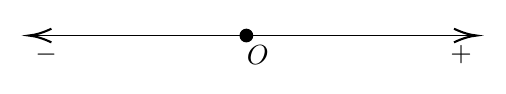
\begin{tikzpicture}[x=0.75pt,y=0.75pt,yscale=-1,xscale=1]
		\draw    (150,111) -- (361.83,111) ;
		\draw [shift={(363.83,111)}, rotate = 180] [color={rgb, 255:red, 0; green, 0; blue, 0 }  ][line width=0.75]    (10.93,-3.29) .. controls (6.95,-1.4) and (3.31,-0.3) .. (0,0) .. controls (3.31,0.3) and (6.95,1.4) .. (10.93,3.29)   ;
		\draw [shift={(148,111)}, rotate = 0] [color={rgb, 255:red, 0; green, 0; blue, 0 }  ][line width=0.75]    (10.93,-3.29) .. controls (6.95,-1.4) and (3.31,-0.3) .. (0,0) .. controls (3.31,0.3) and (6.95,1.4) .. (10.93,3.29)   ;
		\draw  [fill={rgb, 255:red, 0; green, 0; blue, 0 }  ,fill opacity=1 ] (249.83,111) .. controls (249.83,109.32) and (251.19,107.96) .. (252.87,107.96) .. controls (254.55,107.96) and (255.91,109.32) .. (255.91,111) .. controls (255.91,112.68) and (254.55,114.04) .. (252.87,114.04) .. controls (251.19,114.04) and (249.83,112.68) .. (249.83,111) -- cycle ;
		\draw (150,114.4) node [anchor=north west][inner sep=0.75pt]    {$-$};
		\draw (349.83,114.4) node [anchor=north west][inner sep=0.75pt]    {$+$};
		\draw (251.83,114.4) node [anchor=north west][inner sep=0.75pt]    {$O$};
		\end{tikzpicture}	
		\end{center}
	\end{rmk}
\end{df}
Any point in the one dimensional Cartesian system corresponds to a number $\in\R$ and any number $\in\R$ has a location on the line.
The two dimensional Cartesian system is the regular coordinate system. 
\begin{center}
\tikzset{every picture/.style={line width=0.75pt}}      
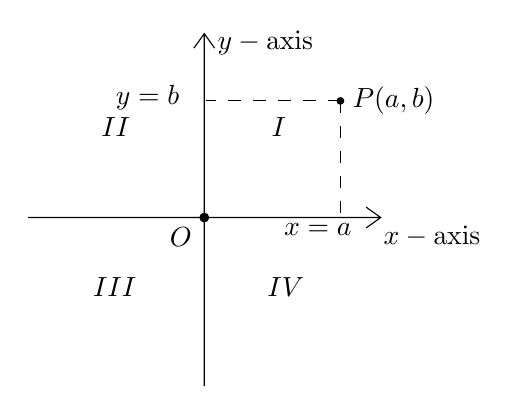
\begin{tikzpicture}[x=0.75pt,y=0.75pt,yscale=-1,xscale=1]
\draw  (50,146.61) -- (219.83,146.61)(134.83,58) -- (134.83,227.83) (212.83,141.61) -- (219.83,146.61) -- (212.83,151.61) (129.83,65) -- (134.83,58) -- (139.83,65)  ;
\draw  [fill={rgb, 255:red, 0; green, 0; blue, 0 }  ,fill opacity=1 ] (198.83,90.41) .. controls (198.83,89.54) and (199.54,88.83) .. (200.41,88.83) .. controls (201.29,88.83) and (202,89.54) .. (202,90.41) .. controls (202,91.29) and (201.29,92) .. (200.41,92) .. controls (199.54,92) and (198.83,91.29) .. (198.83,90.41) -- cycle ;
\draw  [fill={rgb, 255:red, 0; green, 0; blue, 0 }  ,fill opacity=1 ] (132.74,146.61) .. controls (132.74,145.45) and (133.68,144.52) .. (134.83,144.52) .. controls (135.98,144.52) and (136.91,145.45) .. (136.91,146.61) .. controls (136.91,147.76) and (135.98,148.69) .. (134.83,148.69) .. controls (133.68,148.69) and (132.74,147.76) .. (132.74,146.61) -- cycle ;
\draw  [dash pattern={on 4.5pt off 4.5pt}]  (200.41,90.41) -- (200.41,146.61) ;
\draw  [dash pattern={on 4.5pt off 4.5pt}]  (200.41,90.41) -- (135.83,90.41) ;
\draw (166,97.4) node [anchor=north west][inner sep=0.75pt]    {$I$};
\draw (84,97.4) node [anchor=north west][inner sep=0.75pt]    {$II$};
\draw (80,174.4) node [anchor=north west][inner sep=0.75pt]    {$III$};
\draw (164,174.4) node [anchor=north west][inner sep=0.75pt]    {$IV$};
\draw (220,149.4) node [anchor=north west][inner sep=0.75pt]    {$x-\text{axis}$};
\draw (140,55.4) node [anchor=north west][inner sep=0.75pt]    {$y-\text{axis}$};
\draw (205,82.4) node [anchor=north west][inner sep=0.75pt]    {$P( a,b)$};
\draw (117,150.4) node [anchor=north west][inner sep=0.75pt]    {$O$};
\draw (172,148.4) node [anchor=north west][inner sep=0.75pt]    {$x=a$};
\draw (91,81.4) node [anchor=north west][inner sep=0.75pt]    {$y=b$};
\end{tikzpicture}	
\end{center}
The three dimensional Cartesian system includes three perpendicular axes. 
\begin{center}
\tikzset{every picture/.style={line width=0.75pt}}
\begin{tikzpicture}[x=0.75pt,y=0.75pt,yscale=-1,xscale=1]
\draw  (125.83,146.62) -- (219.83,146.62)(135.14,58) -- (135.14,155.06) (212.83,141.62) -- (219.83,146.62) -- (212.83,151.62) (130.14,65) -- (135.14,58) -- (140.14,65)  ;
\draw  [fill={rgb, 255:red, 0; green, 0; blue, 0 }  ,fill opacity=1 ] (132.74,146.61) .. controls (132.74,145.45) and (133.68,144.52) .. (134.83,144.52) .. controls (135.98,144.52) and (136.91,145.45) .. (136.91,146.61) .. controls (136.91,147.76) and (135.98,148.69) .. (134.83,148.69) .. controls (133.68,148.69) and (132.74,147.76) .. (132.74,146.61) -- cycle ;
\draw    (134.83,146.61) -- (72.36,198.78) ;
\draw [shift={(70.83,200.06)}, rotate = 320.13] [color={rgb, 255:red, 0; green, 0; blue, 0 }  ][line width=0.75]    (10.93,-3.29) .. controls (6.95,-1.4) and (3.31,-0.3) .. (0,0) .. controls (3.31,0.3) and (6.95,1.4) .. (10.93,3.29)   ;
\draw (221,149.4) node [anchor=north west][inner sep=0.75pt]    {$y$};
\draw (140,55.4) node [anchor=north west][inner sep=0.75pt]    {$z$};
\draw (134.74,150.01) node [anchor=north west][inner sep=0.75pt]    {$O$};
\draw (72.83,203.46) node [anchor=north west][inner sep=0.75pt]    {$x$};
\end{tikzpicture}	
\end{center}
\begin{df}[Octant]
	A \textbf{Octant} is one of the eight divisions of the three dimensional coordinate system.	
\end{df}
\begin{df}[Hyperplane]
The hyperplane of $y=2$ is given as below: 
	\begin{center}
	\tikzset{every picture/.style={line width=0.75pt}}
	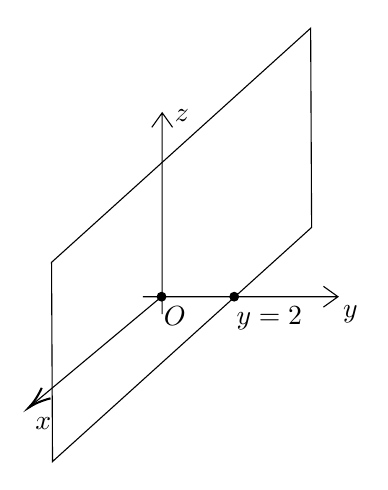
\begin{tikzpicture}[x=0.75pt,y=0.75pt,yscale=-1,xscale=1]
	\draw  (125.83,146.62) -- (219.83,146.62)(135.14,58) -- (135.14,155.06) (212.83,141.62) -- (219.83,146.62) -- (212.83,151.62) (130.14,65) -- (135.14,58) -- (140.14,65)  ;
	\draw  [fill={rgb, 255:red, 0; green, 0; blue, 0 }  ,fill opacity=1 ] (132.74,146.61) .. controls (132.74,145.45) and (133.68,144.52) .. (134.83,144.52) .. controls (135.98,144.52) and (136.91,145.45) .. (136.91,146.61) .. controls (136.91,147.76) and (135.98,148.69) .. (134.83,148.69) .. controls (133.68,148.69) and (132.74,147.76) .. (132.74,146.61) -- cycle ;
	\draw    (134.83,146.61) -- (72.36,198.78) ;
	\draw [shift={(70.83,200.06)}, rotate = 320.13] [color={rgb, 255:red, 0; green, 0; blue, 0 }  ][line width=0.75]    (10.93,-3.29) .. controls (6.95,-1.4) and (3.31,-0.3) .. (0,0) .. controls (3.31,0.3) and (6.95,1.4) .. (10.93,3.29)   ;
	\draw   (206.66,17.26) -- (207.13,113.23) -- (82.3,226.03) -- (81.83,130.06) -- cycle ;
	\draw  [fill={rgb, 255:red, 0; green, 0; blue, 0 }  ,fill opacity=1 ] (167.74,146.61) .. controls (167.74,145.45) and (168.68,144.52) .. (169.83,144.52) .. controls (170.98,144.52) and (171.91,145.45) .. (171.91,146.61) .. controls (171.91,147.76) and (170.98,148.69) .. (169.83,148.69) .. controls (168.68,148.69) and (167.74,147.76) .. (167.74,146.61) -- cycle ;
	\draw (221,149.4) node [anchor=north west][inner sep=0.75pt]    {$y$};
	\draw (140,55.4) node [anchor=north west][inner sep=0.75pt]    {$z$};
	\draw (134.74,150.01) node [anchor=north west][inner sep=0.75pt]    {$O$};
	\draw (72.83,203.46) node [anchor=north west][inner sep=0.75pt]    {$x$};
	\draw (169.74,150.01) node [anchor=north west][inner sep=0.75pt]    {$y=2$};
	\end{tikzpicture}
	\end{center}
	
	Specially: 
	\begin{center}
	\tikzset{every picture/.style={line width=0.75pt}}
	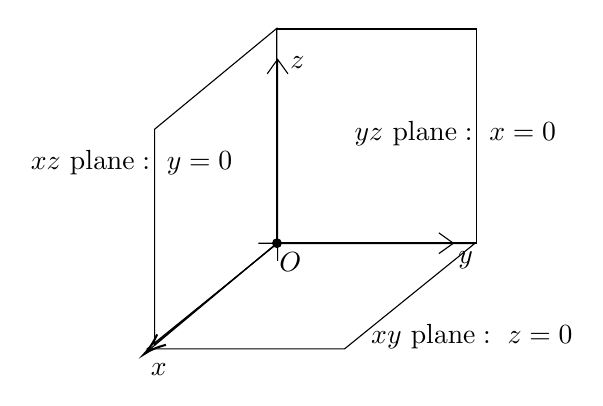
\begin{tikzpicture}[x=0.75pt,y=0.75pt,yscale=-1,xscale=1]
	\draw  (125.83,146.62) -- (219.83,146.62)(135.14,58) -- (135.14,155.06) (212.83,141.62) -- (219.83,146.62) -- (212.83,151.62) (130.14,65) -- (135.14,58) -- (140.14,65)  ;
	\draw  [fill={rgb, 255:red, 0; green, 0; blue, 0 }  ,fill opacity=1 ] (132.74,146.61) .. controls (132.74,145.45) and (133.68,144.52) .. (134.83,144.52) .. controls (135.98,144.52) and (136.91,145.45) .. (136.91,146.61) .. controls (136.91,147.76) and (135.98,148.69) .. (134.83,148.69) .. controls (133.68,148.69) and (132.74,147.76) .. (132.74,146.61) -- cycle ;
	\draw    (134.83,146.61) -- (72.36,198.78) ;
	\draw [shift={(70.83,200.06)}, rotate = 320.13] [color={rgb, 255:red, 0; green, 0; blue, 0 }  ][line width=0.75]    (10.93,-3.29) .. controls (6.95,-1.4) and (3.31,-0.3) .. (0,0) .. controls (3.31,0.3) and (6.95,1.4) .. (10.93,3.29)   ;
	\draw   (134.99,146.79) -- (230.08,146.79) -- (167.39,197.52) -- (72.3,197.52) -- cycle ;
	\draw   (134.83,43.03) -- (134.83,146.61) -- (75.88,195.27) -- (75.88,91.7) -- cycle ;
	\draw   (134.83,43.42) -- (230.83,43.42) -- (230.83,146.52) -- (134.83,146.52) -- cycle ;
	\draw (221,149.4) node [anchor=north west][inner sep=0.75pt]    {$y$};
	\draw (140,55.4) node [anchor=north west][inner sep=0.75pt]    {$z$};
	\draw (134.74,150.01) node [anchor=north west][inner sep=0.75pt]    {$O$};
	\draw (72.83,203.46) node [anchor=north west][inner sep=0.75pt]    {$x$};
	\draw (179,184.4) node [anchor=north west][inner sep=0.75pt]    {$xy\text{ plane} :\ z=0$};
	\draw (15,100.4) node [anchor=north west][inner sep=0.75pt]    {$xz\text{ plane} :\ y=0$};
	\draw (171,86.4) node [anchor=north west][inner sep=0.75pt]    {$yz\text{ plane} :\ x=0$};
	\end{tikzpicture}
	\end{center}
\end{df}
\begin{df}[Points in the Three Dimensional System]
	$P(a,b,c)$ indicates the intersection of the three hyperplanes: $x=a$, $y=b$, and $z=c$.	
	\begin{center}
	\tikzset{every picture/.style={line width=0.75pt}}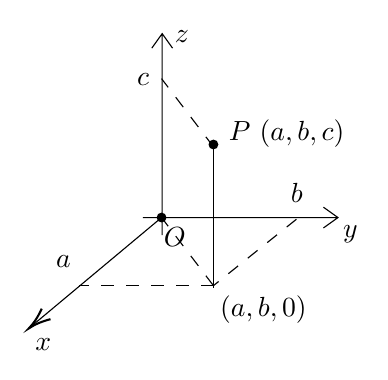
\begin{tikzpicture}[x=0.75pt,y=0.75pt,yscale=-1,xscale=1]
	\draw  (125.83,146.62) -- (219.83,146.62)(135.14,58) -- (135.14,155.06) (212.83,141.62) -- (219.83,146.62) -- (212.83,151.62) (130.14,65) -- (135.14,58) -- (140.14,65)  ;
	\draw  [fill={rgb, 255:red, 0; green, 0; blue, 0 }  ,fill opacity=1 ] (132.74,146.61) .. controls (132.74,145.45) and (133.68,144.52) .. (134.83,144.52) .. controls (135.98,144.52) and (136.91,145.45) .. (136.91,146.61) .. controls (136.91,147.76) and (135.98,148.69) .. (134.83,148.69) .. controls (133.68,148.69) and (132.74,147.76) .. (132.74,146.61) -- cycle ;
	\draw    (134.83,146.61) -- (72.36,198.78) ;
	\draw [shift={(70.83,200.06)}, rotate = 320.13] [color={rgb, 255:red, 0; green, 0; blue, 0 }  ][line width=0.75]    (10.93,-3.29) .. controls (6.95,-1.4) and (3.31,-0.3) .. (0,0) .. controls (3.31,0.3) and (6.95,1.4) .. (10.93,3.29)   ;
	\draw  [fill={rgb, 255:red, 0; green, 0; blue, 0 }  ,fill opacity=1 ] (157.74,111.42) .. controls (157.74,110.27) and (158.68,109.34) .. (159.83,109.34) .. controls (160.98,109.34) and (161.91,110.27) .. (161.91,111.42) .. controls (161.91,112.58) and (160.98,113.51) .. (159.83,113.51) .. controls (158.68,113.51) and (157.74,112.58) .. (157.74,111.42) -- cycle ;
	\draw    (159.83,111.42) -- (159.83,180.42) ;
	\draw  [dash pattern={on 4.5pt off 4.5pt}]  (199.83,147.42) -- (159.83,179.42) ;
	\draw  [dash pattern={on 4.5pt off 4.5pt}]  (159.83,179.42) -- (94.83,179.42) ;
	\draw  [dash pattern={on 4.5pt off 4.5pt}]  (159.83,179.42) -- (134.83,146.61) ;
	\draw  [dash pattern={on 4.5pt off 4.5pt}]  (159.83,112.51) -- (134.83,79.69) ;
	\draw (221,149.4) node [anchor=north west][inner sep=0.75pt]    {$y$};
	\draw (140,55.4) node [anchor=north west][inner sep=0.75pt]    {$z$};
	\draw (134.74,150.01) node [anchor=north west][inner sep=0.75pt]    {$O$};
	\draw (72.83,203.46) node [anchor=north west][inner sep=0.75pt]    {$x$};
	\draw (166,98.4) node [anchor=north west][inner sep=0.75pt]    {$P\ ( a,b,c)$};
	\draw (161.83,182.82) node [anchor=north west][inner sep=0.75pt]    {$( a,b,0)$};
	\draw (82.83,163.82) node [anchor=north west][inner sep=0.75pt]    {$a$};
	\draw (195.83,128.82) node [anchor=north west][inner sep=0.75pt]    {$b$};
	\draw (121.83,75.82) node [anchor=north west][inner sep=0.75pt]    {$c$};
	\end{tikzpicture}
	\end{center}
\end{df}
For spaces in the higher dimension, we understand them via the Cartesian product. 
\begin{df}[Cartesian Product]
	\[\R\times\R\times\cdots\times\R=\{(x_1,\cdots,x_n)|x_i\in\R\forall i=1,\cdots,n\}\] is the set of all $n$-tuples of real numbers and is denoted by $\R^n$.
\end{df}
\begin{eg}
		$(3,4,5)\in\R^3$ is 3 dimensional. $(3,4,5,6)\in\R^4$ is 4 dimensional.	
\end{eg}
\begin{eg}
	Which point(s) $(x,y,z)$ satisfies the equations \[x^2+y^2=1\quad\text{and}\quad x=3? \]	
	\noindent\rule[0.25\baselineskip]{\textwidth}{1pt}
	\begin{center}
	\tikzset{every picture/.style={line width=0.75pt}}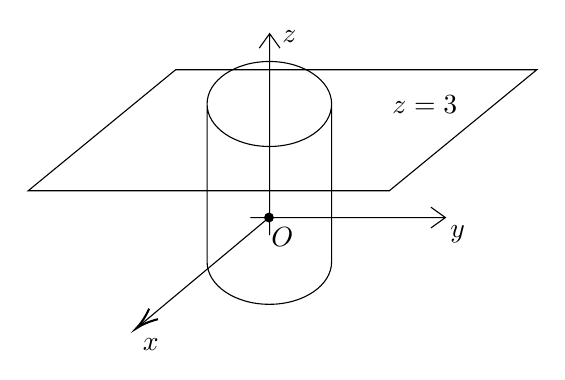
\begin{tikzpicture}[x=0.75pt,y=0.75pt,yscale=-1,xscale=1]
	\draw  (125.83,146.62) -- (219.83,146.62)(135.14,58) -- (135.14,155.06) (212.83,141.62) -- (219.83,146.62) -- (212.83,151.62) (130.14,65) -- (135.14,58) -- (140.14,65)  ;
	\draw  [fill={rgb, 255:red, 0; green, 0; blue, 0 }  ,fill opacity=1 ] (132.74,146.61) .. controls (132.74,145.45) and (133.68,144.52) .. (134.83,144.52) .. controls (135.98,144.52) and (136.91,145.45) .. (136.91,146.61) .. controls (136.91,147.76) and (135.98,148.69) .. (134.83,148.69) .. controls (133.68,148.69) and (132.74,147.76) .. (132.74,146.61) -- cycle ;
	\draw    (134.83,146.61) -- (72.36,198.78) ;
	\draw [shift={(70.83,200.06)}, rotate = 320.13] [color={rgb, 255:red, 0; green, 0; blue, 0 }  ][line width=0.75]    (10.93,-3.29) .. controls (6.95,-1.4) and (3.31,-0.3) .. (0,0) .. controls (3.31,0.3) and (6.95,1.4) .. (10.93,3.29)   ;
	\draw   (165,91.9) -- (165,167.95) .. controls (165,179.26) and (151.57,188.42) .. (135,188.42) .. controls (118.43,188.42) and (105,179.26) .. (105,167.95) -- (105,91.9)(165,91.9) .. controls (165,103.21) and (151.57,112.37) .. (135,112.37) .. controls (118.43,112.37) and (105,103.21) .. (105,91.9) .. controls (105,80.59) and (118.43,71.42) .. (135,71.42) .. controls (151.57,71.42) and (165,80.59) .. (165,91.9) -- cycle ;
	\draw   (89.83,75.42) -- (263.83,75.42) -- (192.83,133.69) -- (18.83,133.69) -- cycle ;
	\draw (221,149.4) node [anchor=north west][inner sep=0.75pt]    {$y$};
	\draw (140,55.4) node [anchor=north west][inner sep=0.75pt]    {$z$};
	\draw (134.74,150.01) node [anchor=north west][inner sep=0.75pt]    {$O$};
	\draw (72.83,203.46) node [anchor=north west][inner sep=0.75pt]    {$x$};
	\draw (193,86.4) node [anchor=north west][inner sep=0.75pt]    {$z=3$};
	\end{tikzpicture}
	\end{center}
	Those points form a circle in the hyperplane of $z=3$ centered at the point $(0,0,3)$ with a radius of $1$.
\end{eg}
\begin{thm}[Distance Formula in Three Dimension]
	For given points $P_1(x_1,y_1,z_1)$ and $P_2(x_2,y_2,z_2)$, the distance between them is denoted by $|P_1P_2|$ and is defined by \[|P_1P_2|=\sqrt{(x_1-x_2)^2+(y_1-y_2)^2+(z_1-z_2)^2}.\]	
\end{thm}
\begin{thm}[Equation of a Sphere]
	An equation of a sphere with a center of $(a,b,c)$ and a radius of $r$ is defined as \[(x-a)^2+(y-b)^2+(z-c)^2=r^2.\]	
\end{thm}
\begin{eg}
	What is the region in $\R^3$ represented by the inequalities \[1\leq x^2+y^2+z^2\leq4\quad\text{and}\quad z\leq0? \]	
	\begin{sol}
	\begin{center}
	\tikzset{every picture/.style={line width=0.75pt}}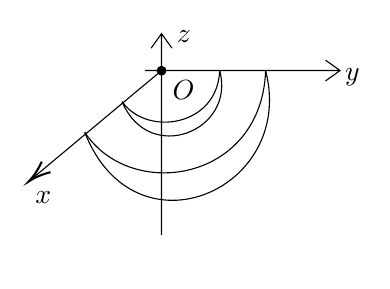
\begin{tikzpicture}[x=0.75pt,y=0.75pt,yscale=-1,xscale=1]
	\draw  (125.83,75.79) -- (219.83,75.79)(133.83,58) -- (133.83,155.06) (212.83,70.79) -- (219.83,75.79) -- (212.83,80.79) (128.83,65) -- (133.83,58) -- (138.83,65)  ;
	\draw  [fill={rgb, 255:red, 0; green, 0; blue, 0 }  ,fill opacity=1 ] (131.74,75.87) .. controls (131.74,74.72) and (132.68,73.79) .. (133.83,73.79) .. controls (134.98,73.79) and (135.91,74.72) .. (135.91,75.87) .. controls (135.91,77.02) and (134.98,77.96) .. (133.83,77.96) .. controls (132.68,77.96) and (131.74,77.02) .. (131.74,75.87) -- cycle ;
	\draw    (133.83,75.79) -- (71.36,127.96) ;
	\draw [shift={(69.83,129.24)}, rotate = 320.13] [color={rgb, 255:red, 0; green, 0; blue, 0 }  ][line width=0.75]    (10.93,-3.29) .. controls (6.95,-1.4) and (3.31,-0.3) .. (0,0) .. controls (3.31,0.3) and (6.95,1.4) .. (10.93,3.29)   ;
	\draw    (114.83,90.79) .. controls (126.83,107.79) and (160.83,102.79) .. (161.83,75.79) ;
	\draw    (114.83,90.79) .. controls (127.83,121.79) and (169.83,104.79) .. (161.83,75.79) ;
	\draw    (96.83,105.54) .. controls (119.08,139.26) and (182.11,129.34) .. (183.97,75.79) ;
	\draw    (96.83,105.54) .. controls (120.93,167.02) and (198.8,133.31) .. (183.97,75.79) ;
	\draw (221,73.4) node [anchor=north west][inner sep=0.75pt]    {$y$};
	\draw (140,55.4) node [anchor=north west][inner sep=0.75pt]    {$z$};
	\draw (137.91,79.27) node [anchor=north west][inner sep=0.75pt]    {$O$};
	\draw (71.83,132.64) node [anchor=north west][inner sep=0.75pt]    {$x$};
	\end{tikzpicture}
	\end{center}
	The region is the difference between the half spheres (the lower half of the sphere) centered at $(0,0,0)$ with a radius of $1$ and $2$.
	\end{sol}
\end{eg}

\subsection{Vectors}
\begin{df}[Vectors]
	\textbf{Vectors} are used to indicate a quantity that has both magnitude and direction. 
	\begin{center}
	\tikzset{every picture/.style={line width=0.75pt}}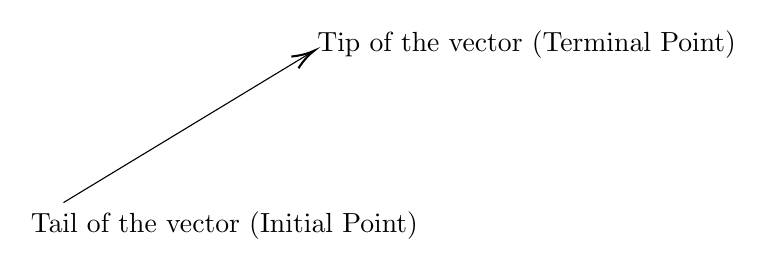
\begin{tikzpicture}[x=0.75pt,y=0.75pt,yscale=-1,xscale=1]
	\draw    (100,124) -- (219.12,51.82) ;
	\draw [shift={(220.83,50.79)}, rotate = 148.79] [color={rgb, 255:red, 0; green, 0; blue, 0 }  ][line width=0.75]    (10.93,-3.29) .. controls (6.95,-1.4) and (3.31,-0.3) .. (0,0) .. controls (3.31,0.3) and (6.95,1.4) .. (10.93,3.29)   ;
	\draw (83,127) node [anchor=north west][inner sep=0.75pt]   [align=left] {Tail of the vector (Initial Point)};
	\draw (221,40) node [anchor=north west][inner sep=0.75pt]   [align=left] {Tip of the vector (Terminal Point)};
	\end{tikzpicture}	
	\end{center}
	\begin{enumerate}
		\item Vectors are denoted as $\vec{v}.$
		\item Magnitude
		\begin{df}[Magnitude]
			A vector is a line segment, of which the \textbf{magnitude} of vector denoted by $|\vec{v}|$ is the length of it and the arrow points the direction of the vector. 
		\end{df}
	\end{enumerate}	
\end{df}
Vectors are operated in a different way: 
\begin{enumerate}
	\item Addition of Vectors: 
	\begin{enumerate}
		\item The triangle law: 
		\begin{center}
		\tikzset{every picture/.style={line width=0.75pt}}
		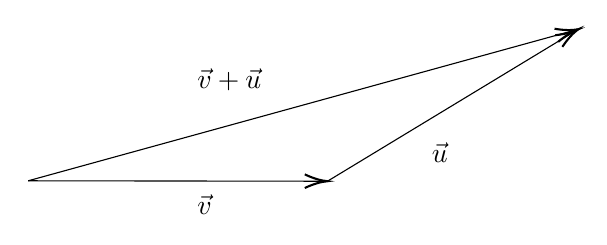
\begin{tikzpicture}[x=0.75pt,y=0.75pt,yscale=-1,xscale=1]
		\draw    (252,160) -- (371.12,87.82) ;
		\draw [shift={(372.83,86.79)}, rotate = 148.79] [color={rgb, 255:red, 0; green, 0; blue, 0 }  ][line width=0.75]    (10.93,-3.29) .. controls (6.95,-1.4) and (3.31,-0.3) .. (0,0) .. controls (3.31,0.3) and (6.95,1.4) .. (10.93,3.29)   ;
		\draw    (107.83,159.79) -- (250,160) ;
		\draw [shift={(252,160)}, rotate = 180.08] [color={rgb, 255:red, 0; green, 0; blue, 0 }  ][line width=0.75]    (10.93,-3.29) .. controls (6.95,-1.4) and (3.31,-0.3) .. (0,0) .. controls (3.31,0.3) and (6.95,1.4) .. (10.93,3.29)   ;
		\draw    (107.83,159.79) -- (370.9,87.32) ;
		\draw [shift={(372.83,86.79)}, rotate = 164.6] [color={rgb, 255:red, 0; green, 0; blue, 0 }  ][line width=0.75]    (10.93,-3.29) .. controls (6.95,-1.4) and (3.31,-0.3) .. (0,0) .. controls (3.31,0.3) and (6.95,1.4) .. (10.93,3.29)   ;
		\draw (188,165.4) node [anchor=north west][inner sep=0.75pt]    {$\vec{v}$};
		\draw (301,140.4) node [anchor=north west][inner sep=0.75pt]    {$\vec{u}$};
		\draw (188,104.4) node [anchor=north west][inner sep=0.75pt]    {$\vec{v} +\vec{u}$};
		\end{tikzpicture}	
		\end{center}
		\item The parallelogram law: 
		\begin{center}
		\tikzset{every picture/.style={line width=0.75pt}}
		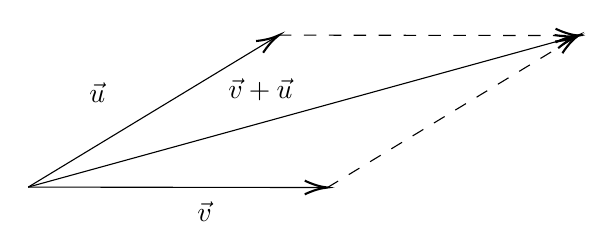
\begin{tikzpicture}[x=0.75pt,y=0.75pt,yscale=-1,xscale=1]
		\draw  [dash pattern={on 4.5pt off 4.5pt}]  (252,160) -- (371.12,87.82) ;
		\draw [shift={(372.83,86.79)}, rotate = 148.79] [color={rgb, 255:red, 0; green, 0; blue, 0 }  ][line width=0.75]    (10.93,-3.29) .. controls (6.95,-1.4) and (3.31,-0.3) .. (0,0) .. controls (3.31,0.3) and (6.95,1.4) .. (10.93,3.29)   ;
		\draw    (107.83,159.79) -- (250,160) ;
		\draw [shift={(252,160)}, rotate = 180.08] [color={rgb, 255:red, 0; green, 0; blue, 0 }  ][line width=0.75]    (10.93,-3.29) .. controls (6.95,-1.4) and (3.31,-0.3) .. (0,0) .. controls (3.31,0.3) and (6.95,1.4) .. (10.93,3.29)   ;
		\draw    (107.83,159.79) -- (370.9,87.32) ;
		\draw [shift={(372.83,86.79)}, rotate = 164.6] [color={rgb, 255:red, 0; green, 0; blue, 0 }  ][line width=0.75]    (10.93,-3.29) .. controls (6.95,-1.4) and (3.31,-0.3) .. (0,0) .. controls (3.31,0.3) and (6.95,1.4) .. (10.93,3.29)   ;
		\draw    (107.83,159.79) -- (226.95,87.61) ;
		\draw [shift={(228.66,86.57)}, rotate = 148.79] [color={rgb, 255:red, 0; green, 0; blue, 0 }  ][line width=0.75]    (10.93,-3.29) .. controls (6.95,-1.4) and (3.31,-0.3) .. (0,0) .. controls (3.31,0.3) and (6.95,1.4) .. (10.93,3.29)   ;
		\draw  [dash pattern={on 4.5pt off 4.5pt}]  (228.66,86.57) -- (370.83,86.78) ;
		\draw [shift={(372.83,86.79)}, rotate = 180.08] [color={rgb, 255:red, 0; green, 0; blue, 0 }  ][line width=0.75]    (10.93,-3.29) .. controls (6.95,-1.4) and (3.31,-0.3) .. (0,0) .. controls (3.31,0.3) and (6.95,1.4) .. (10.93,3.29)   ;
		\draw (188,165.4) node [anchor=north west][inner sep=0.75pt]    {$\vec{v}$};
		\draw (136,108.4) node [anchor=north west][inner sep=0.75pt]    {$\vec{u}$};
		\draw (203,106.4) node [anchor=north west][inner sep=0.75pt]    {$\vec{v} +\vec{u}$};
		\end{tikzpicture}
		\end{center}
	\end{enumerate}
	\item Scalar Multiplications: 
	\begin{center}
	\tikzset{every picture/.style={line width=0.75pt}}
	\begin{tikzpicture}[x=0.75pt,y=0.75pt,yscale=-1,xscale=1]
	\draw    (237.83,126.79) -- (349.03,72.66) ;
	\draw [shift={(350.83,71.79)}, rotate = 154.05] [color={rgb, 255:red, 0; green, 0; blue, 0 }  ][line width=0.75]    (10.93,-3.29) .. controls (6.95,-1.4) and (3.31,-0.3) .. (0,0) .. controls (3.31,0.3) and (6.95,1.4) .. (10.93,3.29)   ;
	\draw [color={rgb, 255:red, 128; green, 128; blue, 128 }  ,draw opacity=1 ]   (237.83,126.79) -- (126.63,180.91) ;
	\draw [shift={(124.83,181.79)}, rotate = 334.05] [color={rgb, 255:red, 128; green, 128; blue, 128 }  ,draw opacity=1 ][line width=0.75]    (10.93,-3.29) .. controls (6.95,-1.4) and (3.31,-0.3) .. (0,0) .. controls (3.31,0.3) and (6.95,1.4) .. (10.93,3.29)   ;
	\draw    (237.83,126.79) -- (292.53,100.16) ;
	\draw [shift={(294.33,99.29)}, rotate = 154.05] [color={rgb, 255:red, 0; green, 0; blue, 0 }  ][line width=0.75]    (10.93,-3.29) .. controls (6.95,-1.4) and (3.31,-0.3) .. (0,0) .. controls (3.31,0.3) and (6.95,1.4) .. (10.93,3.29)   ;
	\draw (352.83,75.19) node [anchor=north west][inner sep=0.75pt]    {$\vec{v}$};
	\draw (166.83,164.19) node [anchor=north west][inner sep=0.75pt]    {$-\vec{v}$};
	\draw (268.08,116.44) node [anchor=north west][inner sep=0.75pt]    {$\frac{1}{2}\vec{v}$};
	\end{tikzpicture}
	\end{center}
	\begin{df}[Scalar Multiplication]
		If $c\in\R$ and $\vec{v}$ is a vector, then $c\vec{v}$ is in the same direction of $\vec{v}$ if $c>0$ and in the opposite direction if $c<0$.
	\end{df}
	\begin{thm}
		The magnitude of $c\vec{v}$: \[|c\vec{v}|=c|\vec{v}|.\]
	\end{thm}
	\item Differences of Vectors: 
	\begin{center}
		\tikzset{every picture/.style={line width=0.75pt}}
	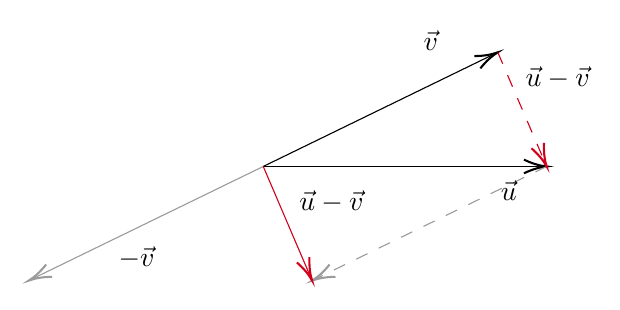
\begin{tikzpicture}[x=0.75pt,y=0.75pt,yscale=-1,xscale=1]
	\draw    (237.83,126.79) -- (349.03,72.66) ;
	\draw [shift={(350.83,71.79)}, rotate = 154.05] [color={rgb, 255:red, 0; green, 0; blue, 0 }  ][line width=0.75]    (10.93,-3.29) .. controls (6.95,-1.4) and (3.31,-0.3) .. (0,0) .. controls (3.31,0.3) and (6.95,1.4) .. (10.93,3.29)   ;
	\draw [color={rgb, 255:red, 155; green, 155; blue, 155 }  ,draw opacity=1 ]   (237.83,126.79) -- (126.63,180.91) ;
	\draw [shift={(124.83,181.79)}, rotate = 334.05] [color={rgb, 255:red, 155; green, 155; blue, 155 }  ,draw opacity=1 ][line width=0.75]    (10.93,-3.29) .. controls (6.95,-1.4) and (3.31,-0.3) .. (0,0) .. controls (3.31,0.3) and (6.95,1.4) .. (10.93,3.29)   ;
	\draw    (237.83,126.79) -- (372.37,126.79) ;
	\draw [shift={(374.37,126.79)}, rotate = 180] [color={rgb, 255:red, 0; green, 0; blue, 0 }  ][line width=0.75]    (10.93,-3.29) .. controls (6.95,-1.4) and (3.31,-0.3) .. (0,0) .. controls (3.31,0.3) and (6.95,1.4) .. (10.93,3.29)   ;
	\draw [color={rgb, 255:red, 155; green, 155; blue, 155 }  ,draw opacity=1 ] [dash pattern={on 4.5pt off 4.5pt}]  (374.37,126.79) -- (263.17,180.91) ;
	\draw [shift={(261.37,181.79)}, rotate = 334.05] [color={rgb, 255:red, 155; green, 155; blue, 155 }  ,draw opacity=1 ][line width=0.75]    (10.93,-3.29) .. controls (6.95,-1.4) and (3.31,-0.3) .. (0,0) .. controls (3.31,0.3) and (6.95,1.4) .. (10.93,3.29)   ;
	\draw [color={rgb, 255:red, 208; green, 2; blue, 27 }  ,draw opacity=1 ]   (237.83,126.79) -- (260.59,179.95) ;
	\draw [shift={(261.37,181.79)}, rotate = 246.82] [color={rgb, 255:red, 208; green, 2; blue, 27 }  ,draw opacity=1 ][line width=0.75]    (10.93,-3.29) .. controls (6.95,-1.4) and (3.31,-0.3) .. (0,0) .. controls (3.31,0.3) and (6.95,1.4) .. (10.93,3.29)   ;
	\draw [color={rgb, 255:red, 208; green, 2; blue, 27 }  ,draw opacity=1 ] [dash pattern={on 4.5pt off 4.5pt}]  (350.83,71.79) -- (373.59,124.95) ;
	\draw [shift={(374.37,126.79)}, rotate = 246.82] [color={rgb, 255:red, 208; green, 2; blue, 27 }  ,draw opacity=1 ][line width=0.75]    (10.93,-3.29) .. controls (6.95,-1.4) and (3.31,-0.3) .. (0,0) .. controls (3.31,0.3) and (6.95,1.4) .. (10.93,3.29)   ;
	\draw (313.83,60.19) node [anchor=north west][inner sep=0.75pt]    {$\vec{v}$};
	\draw (166.83,164.19) node [anchor=north west][inner sep=0.75pt]    {$-\vec{v}$};
	\draw (351,132.4) node [anchor=north west][inner sep=0.75pt]    {$\vec{u}$};
	\draw (254,137.4) node [anchor=north west][inner sep=0.75pt]    {$\vec{u} -\vec{v}$};
	\draw (363,77.4) node [anchor=north west][inner sep=0.75pt]    {$\vec{u} -\vec{v}$};
	\end{tikzpicture}
	\end{center}
 	The difference of vectors $\vecu$ and $\vecv$ is denoted by $\vecu-\vecv$ and is defined by \[\vecu-\vecv=\vecu+(-\vecv)\]
 	\item Properties of vectors: \\Suppose $\veca,\ \vecb,\ \vecc$ are vectors in $V_n$ and $c$ and $d$ are scalars (\textit{Those properties can be proven geometrically}): 
 	\begin{enumerate}
 		\item $\veca+\vecb=\vecb+\veca$
 		\item $\veca+(\vecb+\vecc)=(\veca+\vecb)+\vecc$
 		\item $\veca+0=\veca$
 		\item $\veca+(-\veca)=0$
 		\item $c(\veca+\vecb)=c\veca+c\vecb$
 		\item $(c+d)\veca=c\veca+d\veca$
 		\item $(cd)\veca=c(d\veca)$
 		\item $1\cdot\veca=\veca$
 	\end{enumerate}
\end{enumerate}
We can link the coordinate system and vectors together:  
\begin{enumerate}
	\item \begin{df}[Components of Vectors] We will denote vector $\vecv$ as \[\vecv=\langle a_1,a_2\rangle,\] where $a_1$ and $a_2$ are called the \textbf{components} of $\vecv.$ \end{df}
	\begin{center}
	\tikzset{every picture/.style={line width=0.75pt}} 
	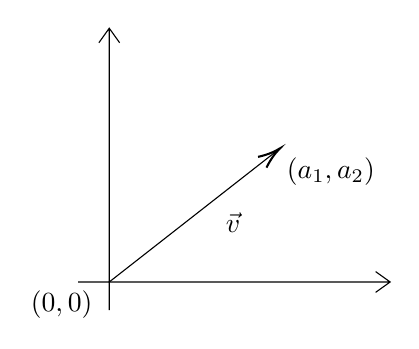
\begin{tikzpicture}[x=0.75pt,y=0.75pt,yscale=-1,xscale=1]
	\draw  (50,191.25) -- (200.37,191.25)(65.04,69) -- (65.04,204.83) (193.37,186.25) -- (200.37,191.25) -- (193.37,196.25) (60.04,76) -- (65.04,69) -- (70.04,76)  ;
	\draw    (65.04,191.25) -- (145.8,128.06) ;
	\draw [shift={(147.37,126.83)}, rotate = 141.96] [color={rgb, 255:red, 0; green, 0; blue, 0 }  ][line width=0.75]    (10.93,-3.29) .. controls (6.95,-1.4) and (3.31,-0.3) .. (0,0) .. controls (3.31,0.3) and (6.95,1.4) .. (10.93,3.29)   ;
	\draw (26,194.4) node [anchor=north west][inner sep=0.75pt]    {$( 0,0)$};
	\draw (149.37,130.23) node [anchor=north west][inner sep=0.75pt]    {$( a_{1} ,a_{2})$};
	\draw (120,156.4) node [anchor=north west][inner sep=0.75pt]    {$\vec{v}$};
	\end{tikzpicture}
	\end{center}
	\item In the three dimension: \[\vecv=\langle a_1,a_2,a_3\rangle\]
	\begin{center}
	\tikzset{every picture/.style={line width=0.75pt}}
	\begin{tikzpicture}[x=0.75pt,y=0.75pt,yscale=-1,xscale=1]
	\draw  (131,163.25) -- (281.37,163.25)(146.04,41) -- (146.04,176.83) (274.37,158.25) -- (281.37,163.25) -- (274.37,168.25) (141.04,48) -- (146.04,41) -- (151.04,48)  ;
	\draw    (146.04,163.25) -- (226.8,100.06) ;
	\draw [shift={(228.37,98.83)}, rotate = 141.96] [color={rgb, 255:red, 0; green, 0; blue, 0 }  ][line width=0.75]    (10.93,-3.29) .. controls (6.95,-1.4) and (3.31,-0.3) .. (0,0) .. controls (3.31,0.3) and (6.95,1.4) .. (10.93,3.29)   ;
	\draw    (146.04,163.25) -- (88.61,236.53) ;
	\draw [shift={(87.37,238.1)}, rotate = 308.09] [color={rgb, 255:red, 0; green, 0; blue, 0 }  ][line width=0.75]    (10.93,-3.29) .. controls (6.95,-1.4) and (3.31,-0.3) .. (0,0) .. controls (3.31,0.3) and (6.95,1.4) .. (10.93,3.29)   ;
	\draw (90,144.4) node [anchor=north west][inner sep=0.75pt]    {$( 0,0,0)$};
	\draw (230.37,102.23) node [anchor=north west][inner sep=0.75pt]    {$( a_{1} ,a_{2} ,a_{3})$};
	\draw (201,128.4) node [anchor=north west][inner sep=0.75pt]    {$\vec{v}$};
	\draw (97,236.4) node [anchor=north west][inner sep=0.75pt]    {$x$};
	\draw (281,169.4) node [anchor=north west][inner sep=0.75pt]    {$y$};
	\draw (127,40.4) node [anchor=north west][inner sep=0.75pt]    {$z$};
	\end{tikzpicture}
	\end{center}
	\item \begin{df} If $A(x_1,y_1,z_1)$ as the tail of vector $\vecv$ and $B(x_1,y_1,z_1)$ as the tip of vector $\vecv$, then \[\overrightarrow{AB}=\langle x_2-x_1,\ y_2-y_1,\ z_2-z_1\rangle\]\[|\overrightarrow{AB}|=\sqrt{(x_2-x_1)^2+(y_2-y_1)^2+(z_2-z_1)^2}\]\end{df}
	\item \begin{thm}If $\vecv=\langle a,b,c\rangle$ and $\vecu=\langle a',b',c'\rangle$, then \[\vecu+\vecv=\langle a'+a,\ b'+b,\ c'+c\rangle\]\[\vecu-\vecv=\langle a'-a,\ b'-b,\ c'-c\rangle\]\[\alpha\vecu=\langle\alpha a',\ \alpha b',\ \alpha c'\rangle,\text{ where }\alpha\text{ is a scalar.}\]\end{thm}
\end{enumerate}

\begin{df}[Standard Basis Vectors]
	In 2-D, $\veci=\langle 1,0\rangle$ and $\vecj=\langle0,1\rangle$; and in 3-D, $\veci=\langle1,0,0\rangle$, $\vecj=\langle0,1,0\rangle$, and $\veck=\langle0,0,1\rangle$ are called the \textbf{standard basis vectors}. 
	\begin{rmk} Any vectors in 2D and 3D can be written as \[\vecv=\langle a,b,c\rangle=a\veci+b\vecj+c\veck.\]\end{rmk}
\end{df}
\begin{df}[Unit Vector]
	A \textbf{unit vector}is a vector of magnitude of $1$. 
	\begin{eg} \[|\veci|=|\vecj|=|\veck|=1\text{ are unit vectors.}\]\end{eg}
	\begin{thm}
		To find a unit vector in the direction of any vector $\vecv$, we use $\displaystyle\frac{1}{|\vecv|}\vecv$. The length of vector $\displaystyle\frac{\vecv}{|\vecv|}$ is $1$ and its direction is the same as $\vecv$.	
	\end{thm}
\end{df}
\begin{eg}
	If the vectors in the figure satisfy $|\vecu|=|\vecv|=1$, and $\vecu+\vecv+\vecw=0$, find $|\vecw|$.
	\begin{center}
	\tikzset{every picture/.style={line width=0.75pt}}
	\begin{tikzpicture}[x=0.75pt,y=0.75pt,yscale=-1,xscale=1]
	\draw    (100,136.1) -- (222.37,136.1) ;
	\draw [shift={(224.37,136.1)}, rotate = 180] [color={rgb, 255:red, 0; green, 0; blue, 0 }  ][line width=0.75]    (10.93,-3.29) .. controls (6.95,-1.4) and (3.31,-0.3) .. (0,0) .. controls (3.31,0.3) and (6.95,1.4) .. (10.93,3.29)   ;
	\draw    (100,136.1) -- (51.89,87.99) ;
	\draw [shift={(50.47,86.57)}, rotate = 45] [color={rgb, 255:red, 0; green, 0; blue, 0 }  ][line width=0.75]    (10.93,-3.29) .. controls (6.95,-1.4) and (3.31,-0.3) .. (0,0) .. controls (3.31,0.3) and (6.95,1.4) .. (10.93,3.29)   ;
	\draw    (100,136.1) -- (52.79,183.31) ;
	\draw [shift={(51.37,184.73)}, rotate = 315] [color={rgb, 255:red, 0; green, 0; blue, 0 }  ][line width=0.75]    (10.93,-3.29) .. controls (6.95,-1.4) and (3.31,-0.3) .. (0,0) .. controls (3.31,0.3) and (6.95,1.4) .. (10.93,3.29)   ;
	\draw   (85.66,136.16) -- (92.8,128.96) -- (100,136.1) -- (92.86,143.3) -- cycle ;
	\draw (61,75.4) node [anchor=north west][inner sep=0.75pt]    {$\vec{u}$};
	\draw (67,174.4) node [anchor=north west][inner sep=0.75pt]    {$\vec{v}$};
	\draw (204,143.4) node [anchor=north west][inner sep=0.75pt]    {$\vec{w}$};
	\end{tikzpicture}
	\end{center}
	\begin{sol}
	Decompose the vectors: 
	\begin{center}
	\tikzset{every picture/.style={line width=0.75pt}} 
	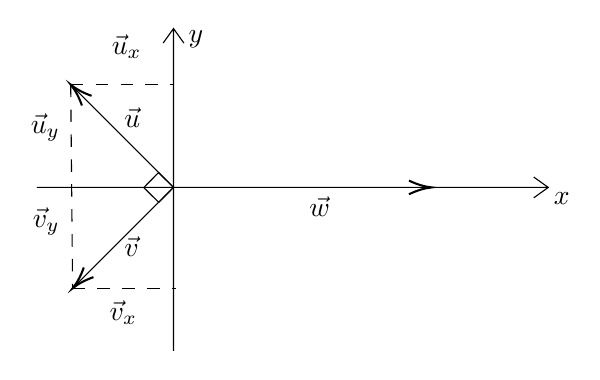
\begin{tikzpicture}[x=0.75pt,y=0.75pt,yscale=-1,xscale=1]
	\draw    (100,136.1) -- (222.37,136.1) ;
	\draw [shift={(224.37,136.1)}, rotate = 180] [color={rgb, 255:red, 0; green, 0; blue, 0 }  ][line width=0.75]    (10.93,-3.29) .. controls (6.95,-1.4) and (3.31,-0.3) .. (0,0) .. controls (3.31,0.3) and (6.95,1.4) .. (10.93,3.29)   ;
	\draw    (100,136.1) -- (51.89,87.99) ;
	\draw [shift={(50.47,86.57)}, rotate = 45] [color={rgb, 255:red, 0; green, 0; blue, 0 }  ][line width=0.75]    (10.93,-3.29) .. controls (6.95,-1.4) and (3.31,-0.3) .. (0,0) .. controls (3.31,0.3) and (6.95,1.4) .. (10.93,3.29)   ;
	\draw    (100,136.1) -- (52.79,183.31) ;
	\draw [shift={(51.37,184.73)}, rotate = 315] [color={rgb, 255:red, 0; green, 0; blue, 0 }  ][line width=0.75]    (10.93,-3.29) .. controls (6.95,-1.4) and (3.31,-0.3) .. (0,0) .. controls (3.31,0.3) and (6.95,1.4) .. (10.93,3.29)   ;
	\draw   (85.66,136.16) -- (92.8,128.96) -- (100,136.1) -- (92.86,143.3) -- cycle ;
	\draw  (34.17,136.1) -- (280.55,136.1)(100,59.56) -- (100,214.82) (273.55,131.1) -- (280.55,136.1) -- (273.55,141.1) (95,66.56) -- (100,59.56) -- (105,66.56)  ;
	\draw  [dash pattern={on 4.5pt off 4.5pt}]  (50.47,86.57) -- (100.37,86.57) ;
	\draw  [dash pattern={on 4.5pt off 4.5pt}]  (50.47,86.57) -- (51.37,184.73) ;
	\draw  [dash pattern={on 4.5pt off 4.5pt}]  (51.37,184.73) -- (101.28,184.73) ;
	\draw (75,96.4) node [anchor=north west][inner sep=0.75pt]    {$\vec{u}$};
	\draw (75,158.4) node [anchor=north west][inner sep=0.75pt]    {$\vec{v}$};
	\draw (164.19,139.5) node [anchor=north west][inner sep=0.75pt]    {$\vec{w}$};
	\draw (282,137.4) node [anchor=north west][inner sep=0.75pt]    {$x$};
	\draw (106,59.4) node [anchor=north west][inner sep=0.75pt]    {$y$};
	\draw (30,99.4) node [anchor=north west][inner sep=0.75pt]    {$\vec{u}_{y}$};
	\draw (31,144.4) node [anchor=north west][inner sep=0.75pt]    {$\vec{v}_{y}$};
	\draw (69,61.4) node [anchor=north west][inner sep=0.75pt]    {$\vec{u}_{x}$};
	\draw (68,189.4) node [anchor=north west][inner sep=0.75pt]    {$\vec{v}_{x}$};
	\end{tikzpicture}
	\end{center}
	We then have \[\cos{45^\circ}=\frac{|\vecu_x|}{\vecu}\Longrightarrow|\vecu_x|=|\vecu|\cos{45^\circ}; \] \[\sin{45^\circ}=\frac{|\vecu_y|}{\vecu}\Longrightarrow|\vecu_y|=|\vecu|\sin{45^\circ}; \]
	\[\begin{aligned}
		\therefore \vecu=\langle|\vecu_x|,\ |\vecu_y\rangle&=-|\vecu_x|\veci+|\vecu_y|\vecj\\
		&=-\frac{\sqrt{2}}{2}|\vecu|\veci+\frac{\sqrt{2}}{2}\vecj\\
		&=\frac{\sqrt{2}}{2}|\vecu|(-\veci+\vecj)
	\end{aligned}\]
	Similarly, \[\vecv=\frac{\sqrt{2}}{2}|\vecv|(-\veci-\vecj).\]
	We know $\vecu+\vecv+\vecw=0$: \[\therefore\vecw+\frac{\sqrt{2}}{2}|\vecu|(-\veci+\vecj)+\frac{\sqrt{2}}{2}|\vecv|(-\veci-\vecj)=0\]
	We know $|\vecu|=|\vecv|=1$: \[\begin{aligned}
		\therefore \vecw+\frac{\sqrt{2}}{2}(-\veci+\vecj)+\frac{\sqrt{2}}{2}(-\veci-\vecj)&=0\\
		\vecw+\frac{\sqrt{2}}{2}(-\veci+\vecj-\veci-\vecj)&=0\\
		\vecw&=\sqrt{2}\veci
	\end{aligned}\]
	\[\therefore \vecw=\langle\sqrt{2},0\rangle\Longrightarrow|\vecw|=\sqrt{2}.\]
	\end{sol}
\end{eg}

\subsection{Dot Product}
\begin{df}[Dot Product]
	If $\vecu=\langle x_1,y_1,z_1\rangle$ and $\vecv=\langle x_2,y_2,z_2\rangle$, then the dot product of $\vecu$ and $\vecv$ is defined as \[\begin{aligned}
		\vecu\cdot\vecv&=\langle x_1,y_1,z_1\rangle\cdot\langle x_2,y_2,z_2\rangle\\
		&=x_1x_2+y_1y_1+z_1z_2 
	\end{aligned}\]	
	\begin{rmk} The dot product of two vectors returns a scalar. \end{rmk}
	\begin{eg}
		Let $\vecu=\veci+2\vecj-3\veck$ and $\vecv=2\vecj-\veck$. Find $\vecu\cdot\vecv$.
		\begin{sol}
			\[\begin{aligned}
			\vecu\cdot\vecv&=\langle1,2,-3\rangle\cdot\langle0,2,-1\rangle\\
				&=(1)(0)+(2)(2)+(-3)(-1)=7.
			\end{aligned}\]	
		\end{sol}
	\end{eg}
\end{df}
Properties of the dot product: 
\begin{enumerate}
	\item $\veca\cdot\vecb=\vecb\cdot\veca$
	\item $\veca\cdot(\vecv+\vecc)=\veca\vecb+\veca\vecc$
	\item $m(\veca\cdot\vecb)=(m\veca)\cdot\vecb=\veca\cdot(m\vecb)=(\veca\cdot\vecb)m$
	\item $\veci\cdot\veci=\vecj\cdot\vecj=\veck\cdot\veck=1$\\$\veci\cdot\vecj=\vecj\cdot\veck=\veck\cdot\veci=0$
\end{enumerate}
\begin{thm}
	\[\vecu\cdot\vecu=|\vecu|^2.\]	
\end{thm}
\begin{thm}
	If $\theta$ is the angle between $\vecu$ and $\vecv$, then \[\boxed{\vecu\cdot\vecv=|\vecu|\cdot|\vecv|\cos\theta}.\]
	\begin{ext} \[\cos\theta=\frac{\vecu\cdot\vecv}{|\vecu||\vecv|}\]\end{ext}
	\begin{ext} \[\theta=90^\circ\Longleftrightarrow\vecu\cdot\vecv=0.\]	\end{ext}
\end{thm}
\begin{df}[Projections]
	We use $\Proj_{\veca}\vecb$ to denote the \textbf{projection} of $\vecb$ on $\veca$.
	\begin{center}
	\tikzset{every picture/.style={line width=0.75pt}}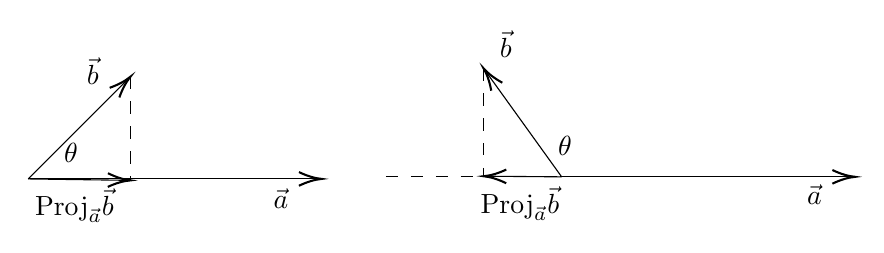
\begin{tikzpicture}[x=0.75pt,y=0.75pt,yscale=-1,xscale=1]
	\draw    (100,118) -- (239.37,118) ;
	\draw [shift={(241.37,118)}, rotate = 180] [color={rgb, 255:red, 0; green, 0; blue, 0 }  ][line width=0.75]    (10.93,-3.29) .. controls (6.95,-1.4) and (3.31,-0.3) .. (0,0) .. controls (3.31,0.3) and (6.95,1.4) .. (10.93,3.29)   ;
	\draw    (100,118) -- (147.89,70.11) ;
	\draw [shift={(149.3,68.7)}, rotate = 135] [color={rgb, 255:red, 0; green, 0; blue, 0 }  ][line width=0.75]    (10.93,-3.29) .. controls (6.95,-1.4) and (3.31,-0.3) .. (0,0) .. controls (3.31,0.3) and (6.95,1.4) .. (10.93,3.29)   ;
	\draw    (357,117) -- (496.37,117) ;
	\draw [shift={(498.37,117)}, rotate = 180] [color={rgb, 255:red, 0; green, 0; blue, 0 }  ][line width=0.75]    (10.93,-3.29) .. controls (6.95,-1.4) and (3.31,-0.3) .. (0,0) .. controls (3.31,0.3) and (6.95,1.4) .. (10.93,3.29)   ;
	\draw    (357,117) -- (320.54,66.32) ;
	\draw [shift={(319.37,64.7)}, rotate = 54.27] [color={rgb, 255:red, 0; green, 0; blue, 0 }  ][line width=0.75]    (10.93,-3.29) .. controls (6.95,-1.4) and (3.31,-0.3) .. (0,0) .. controls (3.31,0.3) and (6.95,1.4) .. (10.93,3.29)   ;
	\draw    (100,118) -- (147.3,118.67) ;
	\draw [shift={(149.3,118.7)}, rotate = 180.81] [color={rgb, 255:red, 0; green, 0; blue, 0 }  ][line width=0.75]    (10.93,-3.29) .. controls (6.95,-1.4) and (3.31,-0.3) .. (0,0) .. controls (3.31,0.3) and (6.95,1.4) .. (10.93,3.29)   ;
	\draw  [dash pattern={on 4.5pt off 4.5pt}]  (149.3,68.7) -- (149.3,118.7) ;
	\draw  [dash pattern={on 4.5pt off 4.5pt}]  (272.37,117) -- (357,117) ;
	\draw  [dash pattern={on 4.5pt off 4.5pt}]  (319.37,64.7) -- (319.37,116.7) ;
	\draw    (357,117) -- (321.37,116.71) ;
	\draw [shift={(319.37,116.7)}, rotate = 0.46] [color={rgb, 255:red, 0; green, 0; blue, 0 }  ][line width=0.75]    (10.93,-3.29) .. controls (6.95,-1.4) and (3.31,-0.3) .. (0,0) .. controls (3.31,0.3) and (6.95,1.4) .. (10.93,3.29)   ;
	\draw (116,99.4) node [anchor=north west][inner sep=0.75pt]    {$\theta $};
	\draw (354,96.4) node [anchor=north west][inner sep=0.75pt]    {$\theta $};
	\draw (217,121.4) node [anchor=north west][inner sep=0.75pt]    {$\vec{a}$};
	\draw (474,119.4) node [anchor=north west][inner sep=0.75pt]    {$\vec{a}$};
	\draw (127,58.4) node [anchor=north west][inner sep=0.75pt]    {$\vec{b}$};
	\draw (326,45.4) node [anchor=north west][inner sep=0.75pt]    {$\vec{b}$};
	\draw (102,121.4) node [anchor=north west][inner sep=0.75pt]    {$\Proj_{\vec{a}}\vec{b}$};
	\draw (316.69,120.4) node [anchor=north west][inner sep=0.75pt]    {$\Proj_{\vec{a}}\vec{b}$};
	\end{tikzpicture}
	\end{center}
	From the diagrams, \[\cos\theta=\frac{|\Proj_{\veca}\vecb|}{|\vecb|}\Longrightarrow|\Proj_{\veca}\vecb=\boxed{|\vecb|\cos\theta}.\]
	We know that \[\begin{aligned}
		\veca\cdot\vecb&=|\veca||\vecb|\cos\theta\\
		\therefore\frac{\veca\cdot\vecb}{|\veca|}&=\boxed{|\vecb|\cos\theta}\\
		\therefore |\Proj_{\veca}\vecb|&=\frac{\veca\cdot\vecb}{|\veca|},\text{ which is a scalar.}
	\end{aligned}\]
	$|\Proj_{\veca}\vecb|$ is called the \textbf{scalar projection} of $\vecb$ on $\veca$.
	\[\Proj_{\veca}\vecb=|\Proj_{\veca}\vecb|\cdot\underbrace{\frac{\veca}{|\veca|}}_{\text{unit vector}}=\frac{\veca\cdot\vecb}{|\veca|}\cdot\frac{\veca}{|\veca|}=\frac{\veca\cdot\vecb}{|\veca|^2}\cdot\veca\]
	$\Proj_{\veca}\vecb$ is called \textbf{projection} of $\vecb$ on $\veca$ and is a vector. 
\end{df}
\begin{eg}
	Find the scalar projection and vector projection of vector $\vecu=\langle1,1,2\rangle$ onto $\vecv=\langle-2,3,1\rangle$.
	\begin{sol}
		\[\Proj_{\vecv}\vecu=\frac{\vecu\cdot\vecv}{|\vecv|^2}\cdot\vecv\ ;\quad |\Proj_{\vecv}\vecu|=\frac{\vecu\cdot\vecv}{|\vecv|}\]
		We need $|\vecv|=\sqrt{4+9+1}=\sqrt{14}$ and $\vecu\cdot\vecv=(1)(-2)+(1)(3)+(2)(1)=3$
		\[\therefore |\Proj_{\vecv}\vecu|=\frac{3}{\sqrt{14}}\]
		\[\Proj_{\vecv}\vecu=\frac{3}{14}\cdot\vecv=\frac{3}{14}\cdot\langle-2,3,1\rangle=\left\langle-\frac{3}{7},\frac{9}{14},\frac{3}{14}\right\rangle.\]
	\end{sol}
\end{eg}

\subsection{Cross Product}
\begin{df}[Cross Product]
	The \textbf{cross product} of $\vecu$ and $\vecv$ is denoted by $\vecu\times\vecv$ and is a vector that is perpendicular to both $\vecu$ and $\vecv$. If $\vecu=\langle x_1,y_1,z_1\rangle$ and $\vecv=\langle x_2,y_2,z_2\rangle$, then 
	\[\begin{aligned}
		\vecu\times\vecv&=\left|\begin{matrix}\veci&\vecj&\veck\\x_1&y_1&z_1\\x_2&y_2&z_2\end{matrix}\right|=y_1z_2\veci+x_2z_1\vecj+x_1y_2\veck-x_2y_1\veck-y_2z_1\veci-x_1z_2\vecj\\
		&=(y_1z_2-y_2z_1)\veci+(z_1x_2-z_2x_1)\vecj+(x_1y_2-x_2y_1)\veck
	\end{aligned}\]
\end{df}
\begin{eg}
	Prove $\vecu\times\vecv$ is perpendicular to both $\vecu$ and $\vecv$.
	\begin{prf}	
		\[\begin{aligned}
			\vecu\cdot(\vecu\times\vecv)&=\langle x_1,y_1,z_1\rangle\cdot\langle y_1z_2-y_2z_1,\ z_1x_2-z_2x_1,\ x_1y_2-x_2y_1\rangle\\
			&=x_1y_1z_2-x_zy_2z_1+x_2y_1z_1-x_1y_1z_2+x_1y_2z_1-x_2y_1z_1=0
		\end{aligned}\]
		\[\therefore \vecu\times\vecv\perp\vecu\]
		Similarly, $\vecv\cdot(\vecu\times\vecv)=0\Longrightarrow\vecu\times\vecv\perp\vecv.$
	\end{prf}
\end{eg}
\begin{thm}
	If $\theta$ is the angle between vectors $\vecu$ and $\vecv$, then \[|\vecu\times\vecv|=|\vecu||\vecv|\sin\theta.\]
	\begin{prf}
		\[\begin{aligned}
			|\vecu\times\vecv|^2&=(y_1z_2-y_2z_1)^2+(z_1x_2-z_2x_1)^2+(x_1y_2-x_2y_1)^2\\
			&=(x_1^2+y_1^2+z_1^2)(x_2^2+y_2^2+z_2^2)-(x_1x_2+y_1y_2+z_1z_2)^2\\
			&=|\vecu|^2|\vecv|^2-(\vecu\cdot\vecv)^2\\
			&=|\vecu|^2|\vecv|^2-|\vecu|^2|\vecv|^2\cos^2\theta\\
			&=|\vecu|^2|\vecv|^2(1-\cos^2\theta)\\
			&=|\vecu|^2|\vecv|^2\sin^2\theta
		\end{aligned}\]
		\[\therefore |\vecu\times\vecv|=|\vecu||\vecv|\sin\theta.\]
	\end{prf}
\end{thm}
\begin{df}[Parallel]
	If two vectors, $\vecu$ and $\vecv$, are parallel to each other, \[\vecu=c\vecv,\] where $c$ is a scalar.
	\begin{thm}
		For two vectors $\vecu$ and $\vecv$, $\vecu\times\vecv=0$ \emph{iff} $\vecu$ and $\vecv$ are parallel to each other.	
	\end{thm}
\end{df}
\begin{thm}
	The length of the cross product, $|\vecu\times\vecv|$, is the area of the parallelogram determined by the vectors $\vecu$ and $\vecv$.	
	\begin{center}
	\tikzset{every picture/.style={line width=0.75pt}}
	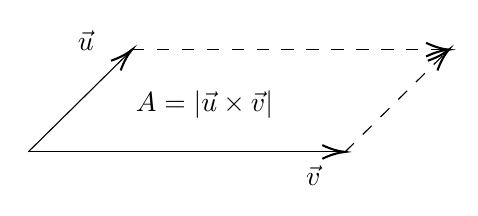
\begin{tikzpicture}[x=0.75pt,y=0.75pt,yscale=-1,xscale=1]
	\draw    (71.37,131) -- (222,131) ;
	\draw [shift={(224,131)}, rotate = 180] [color={rgb, 255:red, 0; green, 0; blue, 0 }  ][line width=0.75]    (10.93,-3.29) .. controls (6.95,-1.4) and (3.31,-0.3) .. (0,0) .. controls (3.31,0.3) and (6.95,1.4) .. (10.93,3.29)   ;
	\draw    (71.37,131) -- (119.95,83.13) ;
	\draw [shift={(121.37,81.73)}, rotate = 135.42] [color={rgb, 255:red, 0; green, 0; blue, 0 }  ][line width=0.75]    (10.93,-3.29) .. controls (6.95,-1.4) and (3.31,-0.3) .. (0,0) .. controls (3.31,0.3) and (6.95,1.4) .. (10.93,3.29)   ;
	\draw  [dash pattern={on 4.5pt off 4.5pt}]  (224,131) -- (272.58,83.13) ;
	\draw [shift={(274,81.73)}, rotate = 135.42] [color={rgb, 255:red, 0; green, 0; blue, 0 }  ][line width=0.75]    (10.93,-3.29) .. controls (6.95,-1.4) and (3.31,-0.3) .. (0,0) .. controls (3.31,0.3) and (6.95,1.4) .. (10.93,3.29)   ;
	\draw  [dash pattern={on 4.5pt off 4.5pt}]  (121.37,81.73) -- (272,81.73) ;
	\draw [shift={(274,81.73)}, rotate = 180] [color={rgb, 255:red, 0; green, 0; blue, 0 }  ][line width=0.75]    (10.93,-3.29) .. controls (6.95,-1.4) and (3.31,-0.3) .. (0,0) .. controls (3.31,0.3) and (6.95,1.4) .. (10.93,3.29)   ;
	\draw (122,100.4) node [anchor=north west][inner sep=0.75pt]    {$A=|\vec{u} \times \vec{v} |$};
	\draw (94,71.4) node [anchor=north west][inner sep=0.75pt]    {$\vec{u}$};
	\draw (204,136.4) node [anchor=north west][inner sep=0.75pt]    {$\vec{v}$};
	\end{tikzpicture}
	\end{center}
\end{thm}
\begin{thm}
	\[\veci\times\vecj=\veck;\quad\vecj\times\veck=\veci;\quad\veck\times\veci=\vecj\]
	\[\vecj\times\veci=-\veck;\quad\veck\times\vecj=-\veci;\quad\veci\times\veck=-\vecj\]
\end{thm}
Properties of cross product ($\veca$, $\vecb$, and $\vecc$ are vectors, and $c$ is a scalar): 
\begin{enumerate}
	\item $\veca\times\vecb=-\vecb\times\veca$
	\item $(c\veca)\times\vecb=c(\veca\times\vecb)=\veca\times(c\vecb)$
	\item $\veca\times(\vecb+\vecc)=\veca\times\vecb+\veca\times\vecc$
	\item $(\veca+\vecb)\times\vecc=\veca\times\vecc+\vecb\times\vecc$
	\item $\veca\cdot(\vecb\times\vecc)=(\veca\times\vecb)\cdot\vecc$
	\item $\veca\times(\vecb\times\vecc)=(\veca\cdot\vecc)\vecb-(\veca\cdot\vecb)\vecc$
\end{enumerate}
\begin{df}[Triple Product]
	The \textbf{scalar triple product} is defined by \[\veca\cdot(\vecb\times\vecc).\]
\end{df}
\begin{thm}
	$|\veca\cdot(\vecb\times\vecc)|$	 denotes the volume of the parallelepiped determined by $\veca$, $\vecb$, and $\vecc$.
	\begin{prf}
		The area of the base is given by \[A=|\vecb\times\vecc|\]
		To find the volume, we need to know the height $h$: \[h=|\veca||\cos\theta|\]
		\[\therefore V=Ah=|\vecb\times\vecc||\veca||\cos\theta|=\veca\cdot(\vecb\times\vecc)\qquad\Big[\vecu\cdot\vecv=|\vecu||\vecv|\cos\theta\Big]\]
		\begin{center}
		\tikzset{every picture/.style={line width=0.75pt}}
		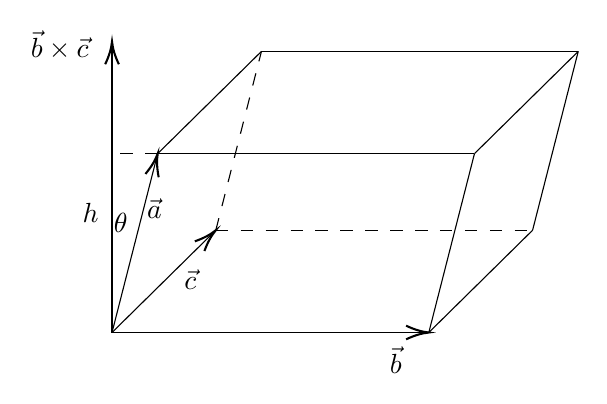
\begin{tikzpicture}[x=0.75pt,y=0.75pt,yscale=-1,xscale=1]
		\draw    (90.37,201) -- (241,201) ;
		\draw [shift={(243,201)}, rotate = 180] [color={rgb, 255:red, 0; green, 0; blue, 0 }  ][line width=0.75]    (10.93,-3.29) .. controls (6.95,-1.4) and (3.31,-0.3) .. (0,0) .. controls (3.31,0.3) and (6.95,1.4) .. (10.93,3.29)   ;
		\draw    (90.37,201) -- (138.95,153.13) ;
		\draw [shift={(140.37,151.73)}, rotate = 135.42] [color={rgb, 255:red, 0; green, 0; blue, 0 }  ][line width=0.75]    (10.93,-3.29) .. controls (6.95,-1.4) and (3.31,-0.3) .. (0,0) .. controls (3.31,0.3) and (6.95,1.4) .. (10.93,3.29)   ;
		\draw    (243,201) -- (293,151.73) ;
		\draw  [dash pattern={on 4.5pt off 4.5pt}]  (140.37,151.73) -- (293,151.73) ;
		\draw    (90.37,201) -- (111.88,116.76) ;
		\draw [shift={(112.37,114.82)}, rotate = 104.32] [color={rgb, 255:red, 0; green, 0; blue, 0 }  ][line width=0.75]    (10.93,-3.29) .. controls (6.95,-1.4) and (3.31,-0.3) .. (0,0) .. controls (3.31,0.3) and (6.95,1.4) .. (10.93,3.29)   ;
		\draw    (112.37,114.82) -- (265,114.82) ;
		\draw    (243,201) -- (265,114.82) ;
		\draw    (112.37,114.82) -- (162.37,65.55) ;
		\draw    (265,114.82) -- (315,65.55) ;
		\draw    (293,151.73) -- (315,65.55) ;
		\draw    (162.37,65.55) -- (315,65.55) ;
		\draw  [dash pattern={on 4.5pt off 4.5pt}]  (140.37,151.73) -- (162.37,65.55) ;
		\draw    (90.37,201) -- (90.37,62.82) ;
		\draw [shift={(90.37,60.82)}, rotate = 90] [color={rgb, 255:red, 0; green, 0; blue, 0 }  ][line width=0.75]    (10.93,-3.29) .. controls (6.95,-1.4) and (3.31,-0.3) .. (0,0) .. controls (3.31,0.3) and (6.95,1.4) .. (10.93,3.29)   ;
		\draw  [dash pattern={on 4.5pt off 4.5pt}]  (112.37,114.82) -- (90.37,114.82) ;
		\draw (124,169.4) node [anchor=north west][inner sep=0.75pt]    {$\vec{c}$};
		\draw (223,206.4) node [anchor=north west][inner sep=0.75pt]    {$\vec{b}$};
		\draw (106,135.4) node [anchor=north west][inner sep=0.75pt]    {$\vec{a}$};
		\draw (50,54.4) node [anchor=north west][inner sep=0.75pt]    {$\vec{b} \times \vec{c}$};
		\draw (90,142.4) node [anchor=north west][inner sep=0.75pt]    {$\theta $};
		\draw (75,137.4) node [anchor=north west][inner sep=0.75pt]    {$h$};
		\end{tikzpicture}
		\end{center}
	\end{prf}
\end{thm}

\subsection{Equations of Lines and Planes}
\begin{thm}[Equation of Lines in 2D]
	If we have a point $P(x_0,y_0)$ and a direction (slope/$\theta$/another point on the line), we have the equation of the line: 
	\[\text{Given }\begin{cases}\text{slope}=m\\P(x_0,y_0)\end{cases}\Longrightarrow\text{ The equation of the line: }y-y_0=m(x-x_0).\]
	\begin{center}
	\tikzset{every picture/.style={line width=0.75pt}}
	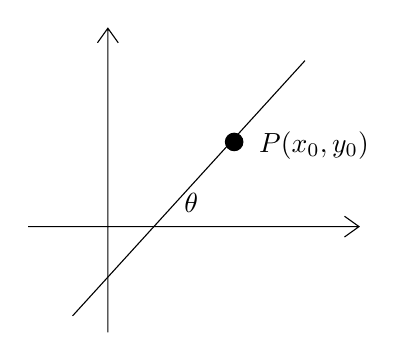
\begin{tikzpicture}[x=0.75pt,y=0.75pt,yscale=-1,xscale=1]
	\draw  (50,166.58) -- (209.37,166.58)(88.37,71) -- (88.37,217.58) (202.37,161.58) -- (209.37,166.58) -- (202.37,171.58) (83.37,78) -- (88.37,71) -- (93.37,78)  ;
	\draw    (183.37,86.58) -- (71.37,209.58) ;
	\draw  [fill={rgb, 255:red, 0; green, 0; blue, 0 }  ,fill opacity=1 ] (145,125.79) .. controls (145,123.46) and (146.89,121.58) .. (149.21,121.58) .. controls (151.54,121.58) and (153.42,123.46) .. (153.42,125.79) .. controls (153.42,128.11) and (151.54,130) .. (149.21,130) .. controls (146.89,130) and (145,128.11) .. (145,125.79) -- cycle ;
	\draw (160,119.4) node [anchor=north west][inner sep=0.75pt]    {$P( x_{0} ,y_{0})$};
	\draw (124,149.4) node [anchor=north west][inner sep=0.75pt]    {$\theta $};
	\end{tikzpicture}
	\end{center}
\end{thm}
\begin{df}[Directional Vector]
	If $\vecv$ is a directional vector of line $L$, \[\veca=t\vecv,\] where $\veca$ is any vector determined by two points on the line. 
\end{df}
\begin{df}[Vector Equations of Lines in 3D]
	Let $\overrightarrow{P_0P}=\veca\Longrightarrow\veca=\langle x-x_0,\ y-y_0\, z-z_0\rangle$
	\begin{center}
	\tikzset{every picture/.style={line width=0.75pt}}
	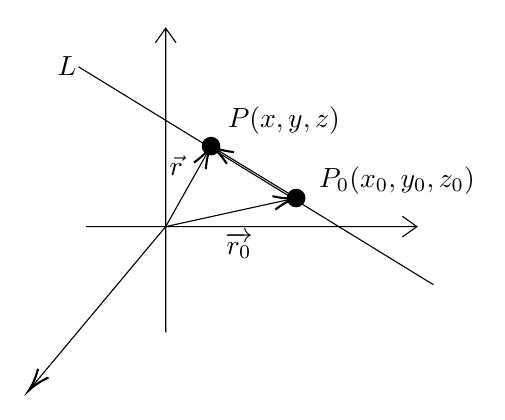
\begin{tikzpicture}[x=0.75pt,y=0.75pt,yscale=-1,xscale=1]
	\draw  (50,166.58) -- (209.37,166.58)(88.37,71) -- (88.37,217.58) (202.37,161.58) -- (209.37,166.58) -- (202.37,171.58) (83.37,78) -- (88.37,71) -- (93.37,78)  ;
	\draw    (217.37,194.58) -- (46.37,89.58) ;
	\draw  [fill={rgb, 255:red, 0; green, 0; blue, 0 }  ,fill opacity=1 ] (147,152.79) .. controls (147,150.46) and (148.89,148.58) .. (151.21,148.58) .. controls (153.54,148.58) and (155.42,150.46) .. (155.42,152.79) .. controls (155.42,155.11) and (153.54,157) .. (151.21,157) .. controls (148.89,157) and (147,155.11) .. (147,152.79) -- cycle ;
	\draw    (88.37,166.58) -- (23.66,244.04) ;
	\draw [shift={(22.37,245.58)}, rotate = 309.88] [color={rgb, 255:red, 0; green, 0; blue, 0 }  ][line width=0.75]    (10.93,-3.29) .. controls (6.95,-1.4) and (3.31,-0.3) .. (0,0) .. controls (3.31,0.3) and (6.95,1.4) .. (10.93,3.29)   ;
	\draw  [fill={rgb, 255:red, 0; green, 0; blue, 0 }  ,fill opacity=1 ] (106,127.79) .. controls (106,125.46) and (107.89,123.58) .. (110.21,123.58) .. controls (112.54,123.58) and (114.42,125.46) .. (114.42,127.79) .. controls (114.42,130.11) and (112.54,132) .. (110.21,132) .. controls (107.89,132) and (106,130.11) .. (106,127.79) -- cycle ;
	\draw    (88.37,166.58) -- (149.26,153.22) ;
	\draw [shift={(151.21,152.79)}, rotate = 167.62] [color={rgb, 255:red, 0; green, 0; blue, 0 }  ][line width=0.75]    (10.93,-3.29) .. controls (6.95,-1.4) and (3.31,-0.3) .. (0,0) .. controls (3.31,0.3) and (6.95,1.4) .. (10.93,3.29)   ;
	\draw    (88.37,166.58) -- (109.23,129.53) ;
	\draw [shift={(110.21,127.79)}, rotate = 119.38] [color={rgb, 255:red, 0; green, 0; blue, 0 }  ][line width=0.75]    (10.93,-3.29) .. controls (6.95,-1.4) and (3.31,-0.3) .. (0,0) .. controls (3.31,0.3) and (6.95,1.4) .. (10.93,3.29)   ;
	\draw    (151.21,152.79) -- (111.92,128.83) ;
	\draw [shift={(110.21,127.79)}, rotate = 31.37] [color={rgb, 255:red, 0; green, 0; blue, 0 }  ][line width=0.75]    (10.93,-3.29) .. controls (6.95,-1.4) and (3.31,-0.3) .. (0,0) .. controls (3.31,0.3) and (6.95,1.4) .. (10.93,3.29)   ;
	\draw (161,136.4) node [anchor=north west][inner sep=0.75pt]    {$P_{0}( x_{0} ,y_{0} ,z_{0})$};
	\draw (117,107.4) node [anchor=north west][inner sep=0.75pt]    {$P( x ,y ,z)$};
	\draw (115.79,168.08) node [anchor=north west][inner sep=0.75pt]    {$\overrightarrow{r_{0}}$};
	\draw (89,131.4) node [anchor=north west][inner sep=0.75pt]    {$\vec{r}$};
	\draw (35,83.4) node [anchor=north west][inner sep=0.75pt]    {$L$};
	\end{tikzpicture}
	\end{center}
	From the diagram, we also have \[\vecr_0+\veca=\vecr.\]
	As $\veca=t\vecv$, \[\vecr=\vecr_0+t\vecv,\]
	which is the \textbf{vector equation} of line $L.$
\end{df}
\begin{thm}
	If $L$ is a line with point $P(x_0,y_0,z_0)$ on it and paralleled to a direction vector $\vecv=\langle a,b,c\rangle$, we have \[\langle x,y,z\rangle=\langle x_0,y_0,z_0\rangle+t\langle a,b,c\rangle,\] where $t$ is a parameter and the equation is called the \textbf{vector equation} of line $L$.	
\end{thm}
\begin{ext}[Parametric Equation of $L$]
	From $\langle x,y,z\rangle=\langle x_0,y_0,z_0\rangle+t\langle a,b,c\rangle,$ we have \[\begin{cases}x=x_0+ta\\y=y_0+tb\\z=z_0+tc\end{cases}\] This system of equations is called the \textbf{parametric equation} of $L$.
\end{ext}
\begin{ext}[Symmetric Equation of $L$]
	From the parametric equation of $L$, we can derive $t$: 
	\[\begin{cases}x=x_0+ta\quad\Longrightarrow\quad t=\frac{x-x_0}{a}\\y=y_0+tb\quad\Longrightarrow\quad t=\frac{y-y_0}{b}\\z=z_0+tc\quad\Longrightarrow\quad t=\frac{z-z_0}{c}\end{cases}\] As $t$ should be equal: \[\frac{x-x_0}{a}=\frac{y-y_0}{b}=\frac{z-z_0}{c},\] which is called the \textbf{symmetric equation} of the line with point $P(x_0,y_0,z_0)$ and a directional vector $\vecv=\langle a,b,c\rangle$.
\end{ext}
\begin{rmk}[Three Forms of Equation of a Line]
	For line $L$ in 3D, $P_0(x_0,y_0,z_0)$ is on $L$ and $\vecv=\langle a,b,c\rangle$ is a directional vector of $L$.
	\begin{enumerate}
		\item The vector form: \[\langle x,y,z\rangle=\langle x_0+ta,\ y_0+tb,\ z_0+tc\rangle\]
		\item The parametric form: \[\begin{cases}x=x_0+ta\\y=y_0+tb\\z=z_0+tc\end{cases}\]
		\item The symmetric form: \[\frac{x-x_0}{a}=\frac{y-y_0}{b}=\frac{z-z_0}{c}\]	
	\end{enumerate}
\end{rmk}
\begin{eg}
	Find the parametric and symmetric equations of the line $L$ passing through the points $(-8,1,4)\quad$ and $\quad (3,-2,4).$
	\begin{sol}
		Let's set $P_0$ to be $(-8,1,4)$ and $P_1$ to be $(3,-2,4).$ So we can find the directional vector \[\vecv=\overrightarrow{P_0P_1}=\langle3-(-8),\ -2-1,\ 4-4\rangle=\langle11,-3,0\rangle.\]
		$\therefore$ The parametric equation of $L$: \[\begin{cases}x=-8+11t\\y=1-3t\\z=4+(0)t\end{cases}, \]
		and the symmetric equation of $L$ is \[\frac{x+8}{11}=\frac{y-1}{-3},\quad z=4.\]
	\end{sol}
\end{eg}
Relationships of two lines in 3D: 
\begin{enumerate}
	\item Parallel: directional vectors of the two lines are parallel to each other.
	\item Intersect: the two lines share one common point
	\item Skewed: the two lines are neither parallel nor intersecting. 
\end{enumerate}
\begin{eg}
	Let \[L_1: \frac{x-2}{1}=\frac{y-3}{-2}=\frac{z-1}{-3}\quad\text{and}\quad L_2: \frac{x-3}{1}=\frac{y+4}{3}=\frac{z-2}{-7}.\] Find the relationship between $L_1$ and $L_2$.
	\begin{sol}
		\[\vecv_1=\langle1,-2,-3\rangle;\quad\vecv_2=\langle1,3,-7\rangle\]	 Because $\vecv_1$ and $\vecv_2$ are not parallel to each other, $L_1$ and $L_2$ are not parallel to each other. \\
		$\therefore$ $L_1$ and $L_2$ can only be intersecting or skewed. \\ 
		To further discuss the relationship between $L_1$ and $L_2$, form parametric equations: 
		\[L_1: \begin{cases}x=2+t\\y=3-2t\\z=1-3t\end{cases}\qquad L_2: \begin{cases}x=3+s\\y=-4+3s\\z=2-7s\end{cases}\]
		If we can find a set of solutions $t$ and $s$ that satisfy the following system of equations, the two lines have point in common and thus is intersecting: \[\begin{cases}2+t=3+s\\3-2t=-4+3s\\1-3t=2-7s\end{cases}\Longrightarrow\begin{cases}t-s=1\quad&\text{\ding{172}}\\2t+3s=7\quad&\text{\ding{173}}\\3t-7s=-1\quad&\text{\ding{174}}\end{cases}\]
		From \ding{172}: \[t=s+1\qquad\text{\ding{175}}\]
		Substitute \ding{173} with \ding{175}: $$\begin{aligned}
			2(s+1)+3s&=7\\
			2s+2+3s&=7\quad\Rightarrow\quad4s=5\quad\Rightarrow\quad s=1\\
			\therefore t=s+1&=1+1=2
		\end{aligned}$$
		Substitute $s=1$ and $t=2$ to \ding{174}: \[\text{LHS}=2(3)-7(1)=6-7=-1=\text{RHS}.\]
		Hence, $\begin{cases}t=2\\s=1\end{cases}$ satisfy all three equations. Substitute $t=2$ to $L_1$: \[x=2+2=4,\quad y=3-2(2)=-1,\quad z=1-3(2)=-5.\]
		$\therefore$ The two lines intersect at $(4,-1,-5).$
	\end{sol}
\end{eg}
\begin{df}[Normal Vector]
	A normal vector is the vector perpendicular to the plane	 and is often denoted as $\vecn$.
\end{df}
\begin{thm}[Vector Equation of a Plane]
	As $\vecn\perp\Pi,$ $\vecn\perp\overrightarrow{P_0P}$
	$$\begin{aligned}
		\overrightarrow{P_0P}&=\vecr-\vecr_0\\
		\therefore\vecn\cdot(\vecr-\vecr_0)&=0\\
		\vecn\cdot\vecr-\vecn\cdot\vecr_0&=0\ \Rightarrow\ \vecn\cdot\vecr=\vecn\cdot\vecr_0,
	\end{aligned}$$
	which is called the \textbf{vector equation} of a plane. 
	\begin{center}
	\tikzset{every picture/.style={line width=0.75pt}}
	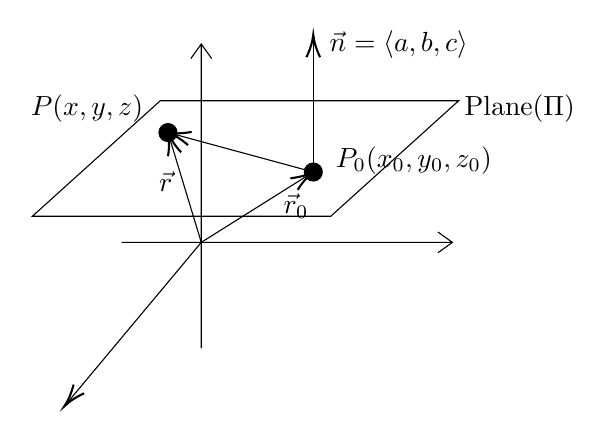
\begin{tikzpicture}[x=0.75pt,y=0.75pt,yscale=-1,xscale=1]
	\draw  (68,124.58) -- (227.37,124.58)(106.37,29) -- (106.37,175.58) (220.37,119.58) -- (227.37,124.58) -- (220.37,129.58) (101.37,36) -- (106.37,29) -- (111.37,36)  ;
	\draw    (106.37,124.58) -- (41.66,202.04) ;
	\draw [shift={(40.37,203.58)}, rotate = 309.88] [color={rgb, 255:red, 0; green, 0; blue, 0 }  ][line width=0.75]    (10.93,-3.29) .. controls (6.95,-1.4) and (3.31,-0.3) .. (0,0) .. controls (3.31,0.3) and (6.95,1.4) .. (10.93,3.29)   ;
	\draw   (86.61,56.34) -- (230.37,56.34) -- (168.76,112) -- (25,112) -- cycle ;
	\draw  [fill={rgb, 255:red, 0; green, 0; blue, 0 }  ,fill opacity=1 ] (156,90.67) .. controls (156,88.28) and (157.94,86.34) .. (160.33,86.34) .. controls (162.72,86.34) and (164.66,88.28) .. (164.66,90.67) .. controls (164.66,93.06) and (162.72,95) .. (160.33,95) .. controls (157.94,95) and (156,93.06) .. (156,90.67) -- cycle ;
	\draw  [fill={rgb, 255:red, 0; green, 0; blue, 0 }  ,fill opacity=1 ] (86,71.67) .. controls (86,69.28) and (87.94,67.34) .. (90.33,67.34) .. controls (92.72,67.34) and (94.66,69.28) .. (94.66,71.67) .. controls (94.66,74.06) and (92.72,76) .. (90.33,76) .. controls (87.94,76) and (86,74.06) .. (86,71.67) -- cycle ;
	\draw    (160.33,90.67) -- (92.26,72.19) ;
	\draw [shift={(90.33,71.67)}, rotate = 15.19] [color={rgb, 255:red, 0; green, 0; blue, 0 }  ][line width=0.75]    (10.93,-3.29) .. controls (6.95,-1.4) and (3.31,-0.3) .. (0,0) .. controls (3.31,0.3) and (6.95,1.4) .. (10.93,3.29)   ;
	\draw    (106.37,124.58) -- (158.64,91.73) ;
	\draw [shift={(160.33,90.67)}, rotate = 147.85] [color={rgb, 255:red, 0; green, 0; blue, 0 }  ][line width=0.75]    (10.93,-3.29) .. controls (6.95,-1.4) and (3.31,-0.3) .. (0,0) .. controls (3.31,0.3) and (6.95,1.4) .. (10.93,3.29)   ;
	\draw    (106.37,124.58) -- (90.91,73.58) ;
	\draw [shift={(90.33,71.67)}, rotate = 73.13] [color={rgb, 255:red, 0; green, 0; blue, 0 }  ][line width=0.75]    (10.93,-3.29) .. controls (6.95,-1.4) and (3.31,-0.3) .. (0,0) .. controls (3.31,0.3) and (6.95,1.4) .. (10.93,3.29)   ;
	\draw    (160.33,90.67) -- (160.33,26.43) ;
	\draw [shift={(160.33,24.43)}, rotate = 90] [color={rgb, 255:red, 0; green, 0; blue, 0 }  ][line width=0.75]    (10.93,-3.29) .. controls (6.95,-1.4) and (3.31,-0.3) .. (0,0) .. controls (3.31,0.3) and (6.95,1.4) .. (10.93,3.29)   ;
	\draw (170,77.4) node [anchor=north west][inner sep=0.75pt]    {$P_{0}( x_{0} ,y_{0} ,z_{0})$};
	\draw (23,52.4) node [anchor=north west][inner sep=0.75pt]    {$P( x ,y ,z)$};
	\draw (144.79,100.08) node [anchor=north west][inner sep=0.75pt]    {$\vec{r}_{0}$};
	\draw (84.79,89.08) node [anchor=north west][inner sep=0.75pt]    {$\vec{r}$};
	\draw (167,21.4) node [anchor=north west][inner sep=0.75pt]    {$\vec{n} =\langle a,b,c\rangle $};
	\draw (232,52.4) node [anchor=north west][inner sep=0.75pt]    {$\text{Plane}( \Pi )$};
	\end{tikzpicture}
	\end{center}
\end{thm}
\begin{ext}[Scalar Equation of a Plane]
	From $\vecn\cdot(\vecr-\vecr_0)=0$: As $\vecn=\langle a,b,c\rangle$ and $\vecr-\vecr_0=\langle x-x_0,\ y-y_0,\ z-z_0\rangle$, we have \[\langle a,b,c\rangle\cdot\langle x-x_0,\ y-y_0,\ z-z_0\rangle=0;\]
	\[\therefore a(x-x_0)+b(y-y_0)+c(z-z_0)=0, \] which is the \textbf{scalar equation} of plane $\Pi$ with point $P_0(x_0,y_0,z_0)$ on it and a normal vector $\vecn=\langle a,b,c\rangle.$
\end{ext}
\begin{ext}[Linear Equation of a Plane]
	From $a(x-x_0)+b(y-y_0)+c(z-z_0)=0$: 
	\[ax+by+cz-(ax_0+by_0+cz_0)=0\]
	Take $d=-(ax_0+by_0+cz_0)$: 
	\[ax+by+cz+d=0,\] which is called the \textbf{linear equation} of plane $\Pi$ with point $P_0(x_0,y_0,z_0)$ on it and a normal vector $\vecn=\langle a,b,c\rangle$.
\end{ext}
\begin{rmk}[Equations of a Plane]
	If point $P_0(x_0,y_0,z_0)$ is on the plane $\Pi$ and a normal vector of $\Pi$ is $\vecn=\langle a,b,c\rangle$: 
	\begin{enumerate}
		\item The vector equation: \[\vecn\cdot\vecr=\vecn\cdot\vecr_0\]
		\item The scalar equation: \[a(x-x_0)+b(y-y_0)+c(z-z_0)=0\]
		\item The linear equation: \[ax+by+cz+d=0,\] where $d=-(ax_0+by_0+cz_0)=-\langle a,b,c\rangle\cdot\langle x_0,y_0,z_0\rangle$
	\end{enumerate}
\end{rmk}
\begin{eg}
	Find an equation of the plane crossing through the points $P(1,3,2)$, $Q(3,-1,6)$, and $R(5,2,0)$.
	\begin{sol}
		Find the normal vector using the following equation: \[			\vecn=\overrightarrow{PQ}\times\overrightarrow{PR}\]
		\[\begin{aligned}
			\overrightarrow{PQ}&=\langle3-1,-1-3,6-2\rangle=\langle2,-4,4\rangle\\
			\overrightarrow{PR}&=\langle5-1,2-3,0-2\rangle=\langle4,-1,-2\rangle
		\end{aligned}\]
		\[\therefore\vecn=\overrightarrow{PQ}\times\overrightarrow{PR}=\left|\begin{matrix}\veci&\vecj&\veck\\2&-4&4\\4&-1&-2\end{matrix}\right|=12\veci+20\vecj+14\veck.\]
		\[\therefore \vecn=\langle12,20,14\rangle,\qquad P(1,3,2)\]
		\[\therefore d=-\langle12,20,14\rangle\cdot\langle1,3,2\rangle=-(12+60+28)=-100.\]
		\[\therefore \text{Linear Equation of } \Pi:\  12x+20y+14z-100=0\quad\Longrightarrow\quad6x+10y+7z-50=0.\]
	\end{sol}
\end{eg}
\begin{thm}[Relationship Between Two Planes]
	If $\vecn_1$ is a normal vector of plane $\Pi_1$, and $\vecn_2$ is a normal vector of plane $\Pi_2$	, then the angle between the two planes is given by \[\theta=\cos^{-1}\left(\frac{\vecn_1\cdot\vecn_2}{|\vecn_1||\vecn_2|}\right).\]
	i.e., the angle between the planes is the angle between the normal vectors. 
\end{thm}
\begin{thm}[Distance from a Point to a Plane]
	Distance of the point $P(x_1,y_1,z_1)$ from the plane $ax+by+cz+d=0$: 
	\begin{equation}\label{d1}
		D=\frac{|ax_a+by_1+cz_1+d|}{\sqrt{a^2+b^2+c^2}} 	
	\end{equation}
	OR
	\begin{equation}\label{d2}
	D=\frac{\vecb\cdot\vecn}{|\vecn|}, 	
	\end{equation}
	where $\vecn$ is the normal vector. 
\end{thm}
\begin{eg}
	Find the distance between the parallel planes: \[\Pi_1:\ 10x+2y-2z=5\quad\text{and}\quad\Pi_2:\ 5x+y-z=1.\]
	\begin{sol}
		Assume point $P(x_1,y_!,z_1)$ is on plane $\Pi_1$: \[\begin{aligned}10x_1+2y_1-2z_1&=5\\\therefore\ 5x_1+y_1-z_1&=\frac{5}{2}\end{aligned}\]	
		Applying formula \ref{d1}: $\vecn=\langle a,b,c\rangle=\langle5,1,-1rlangle,\ d=-1$: 
		\[\therefore\ D=\frac{|5x_1+y_1-z_1+d|}{\sqrt{a^2+b^2+c^2}}=\frac{|\frac{5}{2}-1|}{\sqrt{26+1+1}}=\frac{3/2}{\sqrt{27}}=\frac{3}{2\sqrt{27}}\left(=\frac{\sqrt{3}}{6}\right).\]
	\end{sol}
\end{eg}
\begin{ext}
	Find the distance between two parallel planes: \[\Pi_1:\ ax+by+cz+d=0\quad\text{and}\quad\Pi_2:\ ax+by+cz+d'=0.\]	
	Let point $P(x_1,y_1,z_1)$ on $\Pi_1$: \[ax_1+by_1+cz_1+d=0\]
	Apply formula \ref{d1}: \[D=\frac{|ax_1+by_1+cz_1+d'|}{\sqrt{a^2+b^2+c^2}}=\frac{-d+d'}{\sqrt{a^2+b^2+c^2}}.\]
\end{ext}


\subsection{Cylinders and Quadric Surfaces}
\begin{df}[Cylinders]
	A \textbf{cylinder} is a surface that consists of all lines (called \textbf{rulings}) that are parallel to a given line and pass through a given plane curve. 	
\end{df}
\begin{df}[Quadric Surfaces]
	A \textbf{quadric surface} is the graph of a second-degree equation in three variables $x$, $y$, and $z$. The most general such equation is \[Ax^2+By^2+Cz^2+Dxy+Eyz+Fxz+Gz+Hy+Iz+J=0,\] where $A,B,C,\cdots,J$ are constants, but by translation and rotation it can be brought into one of the standard forms: \[Ax^2+By^2+Cz^2+J=0\quad\text{ or }\quad Ax^2+By^2+Iz=0.\]	
\end{df}
\begin{rmk}
	Graphs of Quadric Surfaces (Refer to Page 877 of the Book): 
	\begin{enumerate}
		\item Ellipsoid: \[\frac{x^2}{a^2}+\frac{y^2}{b^2}+\frac{z^2}{c^2}=1\] All traces are ellipses.\\ If $a=b=c$, the ellipsoid is a sphere.
		\item Elliptic Paraboloid: \[\frac{z}{c}=\frac{x^2}{a^2}+\frac{y^2}{b^2}\] Horizontal traces are ellipses. Vertical traces are parabolas.\\ The variable raised to the first power indicates the axis of the paraboloid. 
		\item Hyperbolic Paraboloid: \[\frac{z}{c}=\frac{x^2}{a^2}-\frac{y^2}{b^2}\] Horizontal traces are hyperbolas. Vertical traces are parabolas.
		\item Cone: \[\frac{z^2}{c^2}=\frac{x^2}{a^2}+\frac{y^2}{b^2}\] Horizontal traces are ellipses.\\ Vertical traces in the planes $x=k$ and $y=k$ are hyperbolas if $k\neq0$ but are pairs of lines if $k=0.$
		\item Hyperboloid of One Sheet: \[\frac{x^2}{a^2}+\frac{y^2}{b^2}-\frac{z^2}{c^2}=1\] Horizontal traces are ellipses. Vertical traces are hyperbolas.\\ The axis of symmetry corresponds to the variable whose coefficient is negative. 
		\item Hyperboloid of Two Sheets: \[-\frac{x^2}{a^2}-\frac{y^2}{b^2}+\frac{z^2}{c^2}=1\] Horizontal traces in $z=k$ are ellipses if $k>c$ or $k<-c$. Vertical traces are hyperbolas.\\ The two minus sign indicate two sheets. 
	\end{enumerate}	
\end{rmk}


\newpage
\section{Vector Functions}
\subsection{Vector Functions and Space Curves}
\begin{df}[Component Functions]
	$f(t),\ g(t),\ h(t)$ are real valued function and are called \textbf{component functions} of $\vecr(t)$. We write \[\vecr(t)=\langle f(t),\ g(t),\ h(t)\rangle=f(t)\veci+g(t)\vecj+h(t)\veck.\]		
\end{df}
\begin{df}[Limit of Vector Functions]
	To find the limit of a vector function, we check its component functions. That is \[\lim_{t\to a}\vecr(t)=\Big\langle\lim_{t\to a}f(t),\ \lim_{t\to a}g(t),\ \lim_{t\to a}h(t)\Big\rangle\]	
\end{df}
\begin{df}[Continuity of Vector Functions]
	A vector function $\vecr(t)$ is continuous if \[\lim_{t\to a}\vecr(t)=\vecr(a).\]	
\end{df}
\begin{eg}
	\begin{enumerate}
		\item Find the domain of \[\vecr(t)=\Big\langle\ln(t+1),\ \frac{t}{\sqrt{9-t^2}},\ 2^t\Big\rangle\]
		\begin{sol}
			\begin{itemize}
				\item Domain of $\ln(t+1)$: $D_1L t+1>0,\ t>-1$
				\item Domain of $\dfrac{t}{\sqrt{9-t^2}}:\ D_2:\ 9-t^2>0,\ -3<t<3$
				\item Domain of $2^t:\ D_3:\ \R$\\
				Find the intersection of domains of component functions: \[D_1\cap D_2\cap D_3:\ -1<t<3\ (t\in(-1,3))\]
			\end{itemize}	
		\end{sol}
		\item Find $\displaystyle\lim_{t\to0}\vecr(t).$
		\begin{sol}
			\[\begin{aligned}
			\lim_{t\to0}\vecr(t)&=\Big\langle\lim_{t\to0}\ln(t+1),\ \lim_{t\to0}\frac{t}{\sqrt{9-t^2}},\ \lim_{t\to0}2^t\Big\rangle\\
			&=\big\langle\ln(1),\ \frac{0}{\sqrt{9}},\ 2^0\big\rangle\\
			&=\langle0,0,1\rangle=\veck
			\end{aligned}\]
		\end{sol}
	\end{enumerate}	
\end{eg}
\begin{eg}
	\[\begin{aligned}
		&\lim_{t\to1}\left(\frac{t^2-t}{t-1}\veci+\sin\pi t\vecj+\cos2\pi t\veck\right)\\
		=&\lim_{t\to1}\left(\frac{t(t-1)}{t-1}\veci+\sin\pi t\vecj+\cos2\pi t\veck\right)\\
		=&\lim_{t\to1}t\veci+\lim_{t\to1}\sin\pi t\vecj+\lim_{t\to1}\cos2\pi t\veck\\
		=&\veci+\sin\pi\vecj+\cos2\pi\veck\\
		=&\veci+\veck
	\end{aligned}\]
\end{eg}
\begin{df}[Graphs of Vector Functions]
	For a vector function $\vecr(t)=f(t)\veci+g(t)\vecj+h(t)\veck$, the graph of it, curve $C$, is defined by the moving tip of the vectors yielded from the vector function. 
	\begin{center}
	\tikzset{every picture/.style={line width=0.75pt}}
	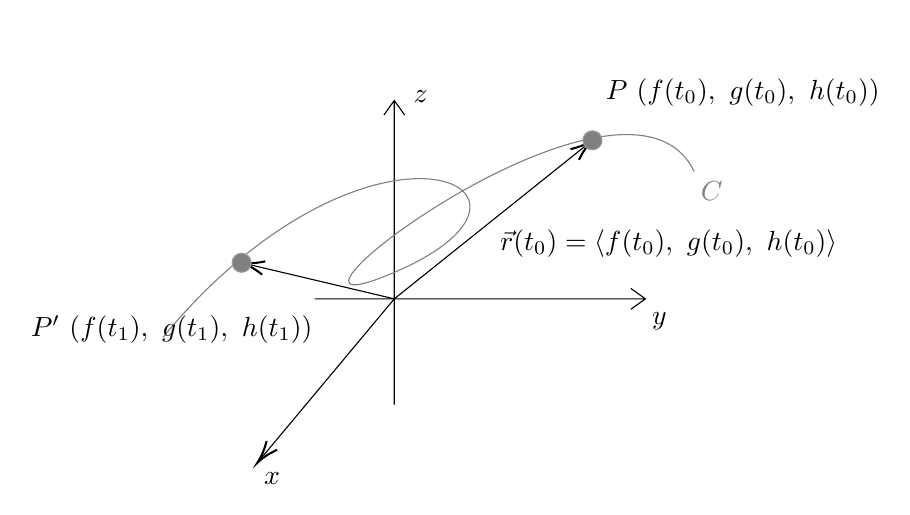
\begin{tikzpicture}[x=0.75pt,y=0.75pt,yscale=-1,xscale=1]
	\draw  (178,160.58) -- (337.37,160.58)(216.37,65) -- (216.37,211.58) (330.37,155.58) -- (337.37,160.58) -- (330.37,165.58) (211.37,72) -- (216.37,65) -- (221.37,72)  ;
	\draw    (216.37,160.58) -- (151.66,238.04) ;
	\draw [shift={(150.37,239.58)}, rotate = 309.88] [color={rgb, 255:red, 0; green, 0; blue, 0 }  ][line width=0.75]    (10.93,-3.29) .. controls (6.95,-1.4) and (3.31,-0.3) .. (0,0) .. controls (3.31,0.3) and (6.95,1.4) .. (10.93,3.29)   ;
	\draw [color={rgb, 255:red, 128; green, 128; blue, 128 }  ,draw opacity=1 ]   (104.82,179.19) .. controls (204.82,58.19) and (308.82,107.19) .. (217.82,147.19) .. controls (126.82,187.19) and (327.82,30.19) .. (360.82,99.19) ;
	\draw    (216.37,160.58) -- (310.26,85.44) ;
	\draw [shift={(311.82,84.19)}, rotate = 141.33] [color={rgb, 255:red, 0; green, 0; blue, 0 }  ][line width=0.75]    (10.93,-3.29) .. controls (6.95,-1.4) and (3.31,-0.3) .. (0,0) .. controls (3.31,0.3) and (6.95,1.4) .. (10.93,3.29)   ;
	\draw  [color={rgb, 255:red, 155; green, 155; blue, 155 }  ,draw opacity=1 ][fill={rgb, 255:red, 128; green, 128; blue, 128 }  ,fill opacity=1 ] (307.23,84.19) .. controls (307.23,81.66) and (309.29,79.6) .. (311.82,79.6) .. controls (314.36,79.6) and (316.41,81.66) .. (316.41,84.19) .. controls (316.41,86.73) and (314.36,88.78) .. (311.82,88.78) .. controls (309.29,88.78) and (307.23,86.73) .. (307.23,84.19) -- cycle ;
	\draw    (216.37,160.58) -- (144.77,143.65) ;
	\draw [shift={(142.82,143.19)}, rotate = 13.3] [color={rgb, 255:red, 0; green, 0; blue, 0 }  ][line width=0.75]    (10.93,-3.29) .. controls (6.95,-1.4) and (3.31,-0.3) .. (0,0) .. controls (3.31,0.3) and (6.95,1.4) .. (10.93,3.29)   ;
	\draw  [color={rgb, 255:red, 155; green, 155; blue, 155 }  ,draw opacity=1 ][fill={rgb, 255:red, 128; green, 128; blue, 128 }  ,fill opacity=1 ] (138.23,143.19) .. controls (138.23,140.66) and (140.29,138.6) .. (142.82,138.6) .. controls (145.36,138.6) and (147.41,140.66) .. (147.41,143.19) .. controls (147.41,145.73) and (145.36,147.78) .. (142.82,147.78) .. controls (140.29,147.78) and (138.23,145.73) .. (138.23,143.19) -- cycle ;
	\draw (317,53.4) node [anchor=north west][inner sep=0.75pt]    {$P\ ( f( t_{0}) ,\ g( t_{0}) ,\ h( t_{0}))$};
	\draw (40,167.4) node [anchor=north west][inner sep=0.75pt]    {$P'\ ( f( t_{1}) ,\ g( t_{1}) ,\ h( t_{1}))$};
	\draw (362.82,102.59) node [anchor=north west][inner sep=0.75pt]  [color={rgb, 255:red, 128; green, 128; blue, 128 }  ,opacity=1 ]  {$C$};
	\draw (152.37,242.98) node [anchor=north west][inner sep=0.75pt]    {$x$};
	\draw (339.37,165.98) node [anchor=north west][inner sep=0.75pt]    {$y$};
	\draw (224.37,58.98) node [anchor=north west][inner sep=0.75pt]    {$z$};
	\draw (266.1,125.79) node [anchor=north west][inner sep=0.75pt]    {$\vec{r}( t_{0}) =\langle f( t_{0}) ,\ g( t_{0}) ,\ h( t_{0}) \rangle $};
	\end{tikzpicture}
	\end{center}
\end{df}
\begin{df}[Space Curve]
	If $f$, $g$, $h$, are continuous real-valued functions on an interval $I$, then the set $C$ of all points $(x,y,z)$ in space $\st$ \[x=f(t)\quad y=g(t)\quad z=h(t),\quad\text{where}t\in I\] is called a \textbf{space curve}.	
\end{df}
\begin{df}[Parametric Equation]
	The system of equations $\begin{cases}x=f(t)\\y=g(y)\\z=h(t)\end{cases}$ is called a \textbf{parametric equation} of $C$ and $t$ is called the \textbf{parameter}.	
\end{df}

\subsection{Derivative and Intergral of Vector Functions}
Limits, continuity, derivative, and integrals of vector functions follow rules similar to those of scalar functions.
\begin{df}[Derivative of Vector Functions]
	\[\frac{\d\vecr}{\d t}=\lim_{h\to0}=\frac{\vecr(t+h)-\vecr(t)}{h},\] $\dfrac{\d\vecr}{\d t}$ or $\vecr'(t)$ is the derivative of $\vecr(t)$ is the limit on the right hand side exists. 
\end{df}
\begin{ext}
	If $\vecr(t)=f(t)\veci+g(t)\vecj+h(t)\veck$, then\[\vecr'(t)=f'(t)\veci+g'(t)\vecj+h'(t)\veck.\]	
\end{ext}
\begin{rmk}[Higher Order Derivatives]
	Higher order derivatives $\dfrac{\d^{(n)}\vecr}{dt^{(n)}}$ can be defined similarly. 	
\end{rmk}
\begin{thm}[Graphic Interpretation of Derivative]
	When $h\to0$, the vector \[\dfrac{\vecr(t+h)-\vecr(t)}{h}\] becomes $\vecr(t)$ and therefore, $\vecr'(t)$ approaches to a vector that lies on the tangent line. $\vecr'(t)$ is called the \textbf{tangent vector}, and \[\vec{T}=\dfrac{\vecr'(t)}{|\vecr'(t)|}\] is called the \textbf{unit tangent vector}.
\end{thm}
\begin{eg}
	Find parametric equations of the tangent line to the vector function $\vecr(t)=\langle2\cos{t},\ \sin{t},\ t\rangle$ at point $(0,1,\dfrac{\pi}{2}).$
	\begin{sol}
		When $t=\frac{\pi}{2}$, $2\cos{\frac{\pi}{2}}=0,\ \sin{\frac{\pi}{2}}=1$.\par $\therefore(0,1,\frac{\pi}{2})$ is on the space curve of $\vecr(t)$.\par Find \[\begin{aligned}\vecr'(t)&=\langle(2\cos{t})',\ (\sin{t})',\ t'\rangle\\&=\langle-2\sin{t},\ \cos{t}, 1\rangle\end{aligned}\]	\par When $t=\frac{\pi}{2}$, \[\vecr'\left(\frac{\pi}{2}\right)=\langle-2\sin{\left(\frac{\pi}{2}\right)},\ \cos{\left(\frac{\pi}{2}\right)}, 1\rangle=\langle-2,0,1\rangle\]\par $\therefore \vecd$ of tangent line $=\langle-2,0,1\rangle$\par \[\therefore\text{Line: }\langle0,1,\frac{\pi}{2}\rangle+\langle-2,0,1\rangle t=\langle-2t,1,\frac{\pi}{2}+t\rangle\]
	\end{sol}	
\end{eg}
\begin{eg}
	If $\vecr(t)=(t^3+2t)\veci-3e^{-2t}\vecj+2\sin{5t}\veck$. Find $\dfrac{\d\vecr}{\d t},\ \left|\dfrac{\d\vecr}{\d t}\right|,\ \dfrac{\d^2\vecr}{\d t^2},\ \left|\dfrac{\d^2\vecr}{\d t^2}\right|.$	
	\begin{sol}
		\[\dfrac{\d\vecr}{\d t}=\langle3t^2+2,\ 6e^{-2t},\ 10\cos{5t}\rangle\]
		\[\dfrac{\d^2\vecr}{\d t^2}=\langle6t,\ -12e^{-2t},\ -50\sin{5t}\rangle\]	
		When $t=0$: 
		\[\vecr'(0)=\langle2,\ 6,\ 10\rangle;\qquad\vecr''(0)=\langle0,\ -12,\ 0\rangle\]
		\[\therefore|\vecr'(0)|=\sqrt{4+36+100}=\sqrt{140}(=2\sqrt{70});\quad|\vecr''(0)|=\sqrt{144}=12.\]
	\end{sol}
\end{eg}
\begin{thm}[Properties of Differentiation]
	\[\ddt[\vecr_1(t)+\vecr_2(t)]=\ddt[\vecr_1(t)]+\ddt[\vecr_2(t)]\]
	\[\ddt[\alpha\vecr(t)]=\alpha\ddt[\vecr(t)]\]
	\[\ddt[f(t)\vecr(t)]=f'(t)\vecr(t)+f(t)\vecr'(t)\]
	\[\ddt[\vecr_1(t)\cdot\vecr_2(t)]=\vecr_1'(t)\cdot\vecr_2(t)+\vecr_1(t)\cdot\vecr_2'(t)\]
	\[\ddt[\vecr_1(t)\times\vecr_2(t)]=\vecr_1'(t)\times\vecr_2(t)+\vecr_1(t)\times\vecr_2'(t)\]	
\end{thm}
\begin{eg}
	Show that if a curve lies on a sphere with center at the origin, then $\vecr'(t)$ is perpendicular to $\vecr(t)$ for any $t$. 
	\begin{sol}
		Let $\vecr(t)$ lies on a sphere, with center at the origin, and radius $R=c$: \[\therefore\vecr(t)=\langle x(t), y(t), z(t)\rangle\quad\text{ and }\quad x^2(t)+y^2(t)+z^2(t)=c^2\]
		\[x^2(t)+y^2(t)+z^2(t)=|\vecr(t)|^2=\vecr(t)\cdot\vecr(t)\]
		\[\therefore\vecr(t)\cdot\vecr(t)=c^2\]\par
		Take derivative of the both sides of the euqation \[\ddt[\vecr(t)\cdot\vecr(t)]=\ddt(c^2)\]
		\[\therefore\vecr'(t)\cdot\vecr(t)+\vecr(t)\cdot\vecr'(t)=0\implies2\vecr'(t)\cdot\vecr(t)=0\]
		\[\therefore\vecr'(t)\cdot\vecr(t)=0\implies\vecr'(t)\perp\vecr(t).\]
	\end{sol}
\end{eg}
\begin{df}[Definite Integral of a Vector Function]
	The definite integral of a continuous vector function $\vecr(t)$ can be defined as \[\int_a^b\vecr(t)\d t=\int_a^bf(t)\d t\veci+\int_a^bg(t)\d t\vecj+\int_a^bh(t)\d t\veck, \] if $\vecr(t)=\Big\langle f(t), g(t), h(t)\Big\rangle.$
\end{df}
\begin{eg}
	\[\begin{aligned}
	\int_0^1\left(\frac{1}{t+1}\veci+\frac{1}{t^2+1}\vecj+\frac{t}{t^2+1}\veck\right)\d t&=\int_0^1\frac{1}{t+1}\d t\veci+\int_0^1\frac{1}{t^2+1}\d t\vecj+\int_0^1\frac{t}{t^2+1}\d t\veck\\
	&=\Bigg[\frac{1}{t+1}\Bigg]_0^1\veci+\Bigg[\frac{1}{t^2+1}\Bigg]_0^1\vecj+\Bigg[\frac{t}{t^2+1}\Bigg]_0^1\veck\\
	&=\ln(2)\veci+\frac{\pi}{4}\vecj+\frac{1}{1}(\ln(2))\veck
	\end{aligned}\]	
\end{eg}

\newpage
\section{Partial Derivative}
\subsection{Function of Several Variables}
\begin{df}[Multivariable Functions]
	A function of $f$ of $n$ variables is a function that takes any $n$-tuple $(x_1,\cdots,x_n)$ in the set $D$ to a number in $\R$, where \[D=\bigg\{(x_1,\cdots,x_n)|x_i\in\R\text{ and }f\text{ is defined in }(x_1,\cdots,x_n)\bigg\}\]	
	\begin{eg}
		$f(x,y)=\sqrt{x^2+y^2-4}$: $f:\begin{array}{l}\R^2\longrightarrow\R\\ (x,y)\longmapsto\text{ a number like }r\end{array}$	
		
		Domain of $f$: all $(x,y)\in\R\emph{ s.t. }x^2+y^2-4\geq0.$ (i.e., Everything exclude the circle centered at the origin with a radius of $2$.)
	\end{eg}
\end{df}
\begin{df}[Graphs of a Two-Variable Function]
	The graph of a two-variable function with domain $D$ is the set of all points $(x,y,z)\in\R^3$ \emph{s.t.} $z=f(x,y)$ and $(x,y)\in D$.	
\end{df}
\begin{df}[Vector Functions]
	\[\vecr:\begin{array}{l}\R\longrightarrow V_n\\ t\longmapsto\langle f(t),\ g(t),\ h(t),\cdots\rangle\end{array}, \] where $V_n$ is a set of all vectors with $n$ components, and $t$ is a parameter. 
	\begin{rmk}
		We will only work with $V_3$, i.e., 	$\vecr:\begin{array}{l}\R\longrightarrow V_3\\ t\longmapsto\langle f(t),\ g(t),\ h(t)\rangle\end{array}$.
	\end{rmk}
\end{df}
\begin{thm}
	A multivariable function creates a surface in the space. if two surfaces intersect each other, then the intersection identifies a curve.	
\end{thm}
\begin{eg}
	Find a vector function $\vecr(t)$ that represents the curve of intersection of two surfaces\[z=\sqrt{x^2+y^2}\qquad\text{and}\qquad z=3+y.\]
	\begin{sol}
		Solve the system of equation $\begin{cases}x=\sqrt{x^2+y^2}\\z=3+y\end{cases}.$\par
		Hence, \[\begin{aligned}
			\sqrt{x^2+y^2}&=3+y\\
			x^2+y^2&=(3+y)^2=y^2+6y+9\\
			x^2&=6y+9\\
			y&=\frac{x^2-9}{6}\\
			\therefore z=&3+y=\frac{x^2+0}{6}
 		\end{aligned}\]\par 
 		Let $x=t$: \[\vecr(t)=\langle x,t,z\rangle=\Big\langle t,\ \frac{t^2-9}{6},\ \frac{t^2+9}{6}\Big\rangle\]
	\end{sol}
\end{eg}
\begin{eg}
	Do the same for surfaces\[z=3x^2+y^2\qquad\text{and}\qquad y=5x^2\]
	\begin{sol}
		Solve the system of equations $\begin{cases}z=3x^2+y^2\\y=5x^2\end{cases}.$\par
		\[\therefore 5x^2=3x^2+y^2\ \Longrightarrow\ z=3x^2+(5x^2)^2=3x^2+25x^4\]\par 
		Let $x=t$: \[\vecr(t)=\langle x,t,z\rangle=\Big\langle t,\ 5t^2,\ 3t^2+25t^4\Big\rangle\]	
	\end{sol}
\end{eg}
\begin{df}[Level Curves]
	The level curve of a two variable function $z=f(x,y)$ is a curve $f(x,y)=k$ (in the $xy$-plane). That means all values of $x$ and $y$ that have the same value $z=k.$
\end{df}
\begin{thm}[Application of Level Curve]
	Given that a point $(a,b)$ is on the level curve of $f(x,y)$ for $k=c$, then we know $f(a,b)=c.$	
\end{thm}

\subsection{Limit and Continuity}
\begin{df}[Limit]
	For two variable function $z=f(x,y)$, we check limit when $(x,y)\to(a,b)$. Therefore, we can make $(x,y)$ closer to $a(b)$ from infinitely many directions. Therefore, \[\lim_{(x,y)\to(a,b)}f(x,y)=L\] if in all directions that $(x,y)$ approaches to $(a,b)$, we have $f(x,y)\to L$.	
\end{df}
\begin{df}[Precise Definition of Limit]
	$\forall$ given $\varepsilon>0$, $\exists$ associated $\delta>0\st$ if $(x,y)\in D$ and $d((x,y),(a,b))<\delta\implies d(f(x,y),L)<\varepsilon,$ where $d((x,y),(a,b))$ is the distance between $(x,y)$ and $(a,b)$ and is calculated by $\sqrt{(x-a)^2+(y-b)^2}.$
\end{df}
\begin{eg}
	Consider function $f(x,y)=\dfrac{xy}{x^2+y^2}$, and identify if it is has a limit at $(0,0)$ or not. 
	\begin{sol}
		In the direction of $x$-axis ($y=0$), we have $f(x,y)=\dfrac{x\cdot0}{x^2+0^2}=0$ and $\displaystyle\lim_{(x,y)\to(0,0)}f(,y)=0$ along the $x$-axis.\par In the direction of $y$-axis ($x=0$), we have $f(x,y)=0.$, and $\displaystyle\lim_{(x,y)\to(0,0)}f(x,y)=0$ along the $y$-axis.\par If $y=x$, $f(x,y)=f(x,x)=\dfrac{x^2}{x^2+x^2}=\dfrac{1}{2}$, and $\displaystyle\lim_{(x,y)\to(0,0)}f(x,y)=\dfrac{1}{2}$ along the line $y=x.$
	\end{sol}
\end{eg}
\begin{eg}
	Find $\displaystyle\lim_{(x,y)\to(0,0)}\frac{x^2y}{x^2+y^2}.$
	\begin{sol}
		By looking at the graph of the function, we think it has a limit at $(0,0)$. This is not enough, and later we will be able to say that limit exists by converting it to polar coordinate.\par Let $y=mx$: \[f(x,y)=f(x,mx)=\frac{x^2\cdot mx}{x^2+(mx)^2}=\frac{x^3m}{x^2(1+m^2)}=\frac{m}{1+m^2}x\]\[\therefore\lim_{(x,y)\to(0,0)}f(x,y)=0\text{ along the line of }y=mx.\]
	\end{sol}
\end{eg}
\begin{eg}
	\[\lim_{(x,y)\to(0,0)}\frac{xy^2}{x^2+y^2}=0\]	
	\[\lim_{(x,y)\to(0,0)}\frac{x^2y}{x^2+y^4}=0\]
	\[\lim_{(x,y)\to(0,0)}\frac{3x^3y}{x^4+y^4}\ \DNE \left(\text{check }\begin{cases}x=0\\y=x\end{cases}\right)\]
\end{eg}
\begin{df}[Continuity]
	Functions of two-variables is continues at $(a,b)$ if \[\lim_{(x,y)\to(a,b)}=f(a,b).\]
\end{df}
\begin{eg}
	Find $\displaystyle\lim_{(x,y)\to(1,2)}(x^2y^3-x^3y^2+3x+2y).$
	\begin{sol}
		As $x^2y^3-x^3y^2+3x+2y$ is a polynomial and continuous everywhere, so 
		\[\lim_{(x,y)\to(1,2)}(x^2y^3-x^3y^2+3x+2y)=(1)^2(2)^3-(1)^3(2)^2
		+3(1)+2(2)=1.\]
	\end{sol}
\end{eg}
\begin{eg}
	$f(x,y)=\dfrac{x^2y}{x^2+y^2}$ is not continuous at $(0,0)$, but \[g(x,y)=\begin{cases}\dfrac{x^2y}{x^2+y^2}\qquad &(x,y)\neq(0,0)\\0\qquad &(x,y)=(0,0)\end{cases}\text{ is continuous at }(0,0).\]
\end{eg}

\subsection{Partial Function}
In two-variable functions, we will have partial derivatives $f_x$ (derivative with respect to $x$) and $f_y$ (derivative with respect to $y$).
\begin{df}[Partial Derivative]
	If $f(x,y)$ is a two variable function, then its partial derivatives are $f_x$ and $f_y$ and is defined as \[\pdfdx=f_x(x,y)=\lim_{h\to0}\frac{f(x+h,y)-f(x,y)}{h}\]\[\pdfdy=f_y(x,y)=\lim_{h\to0}\frac{f(x,y+h)-f(x,y)}{h}\]	
\end{df}
\begin{eg}
	Let $f(x,y)=x^3+x^2y^3-2y$ and find $f_x(2,1)$ and $f_y(2,1)$
	\begin{sol}
		Find $f_x(x,y)$: keep $y$ constant.\par $f_x(x,y)=3x^2+2xy^3$\par \[\therefore f_x(2,1)=3(2)^2+2(2)(1)^3=16\]\par Find $f_y(x,y)$: keep $x$ constant.\par $f_y(x,y)=3x^2y^2-2$\par\[\therefore f_y(2,1)=3(2)^2(1)^2-2=10\]
	\end{sol}
\end{eg}
\begin{eg}
	Let $f(x,y)=4-x^2-2y^2$. Find $f_x(1,1)$ and interpret the values. 
	\begin{sol}
	\begin{center}
	\tikzset{every picture/.style={line width=0.75pt}}
	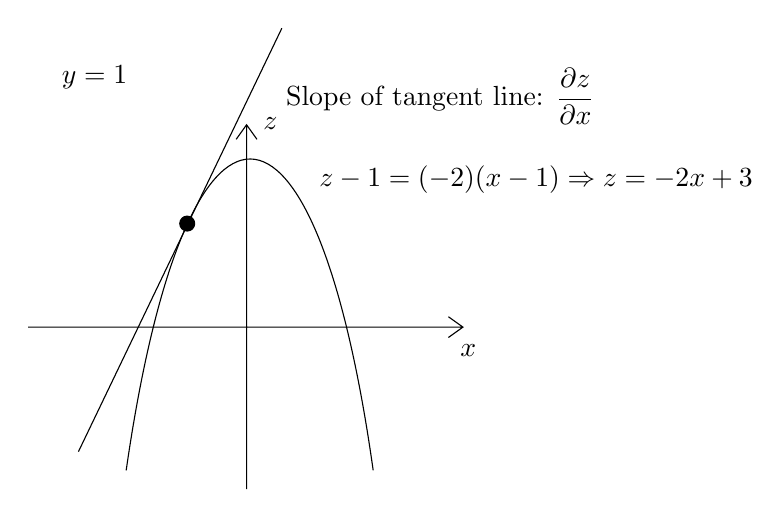
\begin{tikzpicture}[x=0.75pt,y=0.75pt,yscale=-1,xscale=1]
	\draw  (234,181.48) -- (443.44,181.48)(339.19,84) -- (339.19,259.48) (436.44,176.48) -- (443.44,181.48) -- (436.44,186.48) (334.19,91) -- (339.19,84) -- (344.19,91)  ;
	\draw    (281.19,250.48) .. controls (310.19,49.48) and (372.19,51.48) .. (400.19,250.48) ;
	\draw  [fill={rgb, 255:red, 0; green, 0; blue, 0 }  ,fill opacity=1 ] (307,131.59) .. controls (307,129.61) and (308.61,128) .. (310.59,128) .. controls (312.58,128) and (314.19,129.61) .. (314.19,131.59) .. controls (314.19,133.58) and (312.58,135.19) .. (310.59,135.19) .. controls (308.61,135.19) and (307,133.58) .. (307,131.59) -- cycle ;
	\draw    (356.19,37.48) -- (258.19,241.48) ;
	\draw (357,55.4) node [anchor=north west][inner sep=0.75pt]    {$\text{Slope of tangent line: }\dfrac{\partial z}{\partial x}$};
	\draw (373,102.4) node [anchor=north west][inner sep=0.75pt]    {$z-1=( -2)( x-1) \Rightarrow z=-2x+3$};
	\draw (249,54.4) node [anchor=north west][inner sep=0.75pt]    {$y=1$};
	\draw (346,79.4) node [anchor=north west][inner sep=0.75pt]    {$z$};
	\draw (441,188.4) node [anchor=north west][inner sep=0.75pt]    {$x$};
	\end{tikzpicture}
	\end{center}
		$f(1,1)=4-1-2=1\implies A(1,1,1)$ lies on $f(x,y).$\par $\displaystyle\pdfdx=-2x\implies\pdfdx(1,1)=-2$\par Let's consider $y=1$:\par The plane $y=1$ will intersect with $f(x,y)$ at a line $\vecr(t)$.\par Solve $\vecr(t):\ \begin{cases}z=4-x^2-2y^2\\y=1\end{cases}$\par \[\Rightarrow z=4-x^2-2=2-x^2\]\par \[\therefore \vecr(t)=\langle t,1,2-t^2\rangle,\ \vecr'(t)=\langle 1,0,-2t\rangle\]\par At point $A(1,1,1)$, $t=1$.\par $\qquad\therefore\vecr'(1)=\langle1,0,-2\rangle,$ which is a directional vector of the tangent line. \par $\therefore$ Tangent line: \[L:\ x=1+t,\ y=1,\ z=1-2t\]
	\end{sol}
\end{eg}
\begin{df}[Higher Order Partial Derivative]
	\[\pdfdxdx=\pddx\left(\pdfdx\right)\]
	\[\pdfdydy=\pddy\left(\pdfdy\right)\]
	\[\pdfdxdy=\pddx\left(\pdfdy\right)\]
	\[\pdfdydx=\pddy\left(\pdfdx\right)\]
\end{df}
\begin{thm}[Clairaut's Theorem]
	If $f$ is continuous on a disk $D$, then \[\pdfdxdy=\pdfdydx.\]
\end{thm}
\begin{df}[Functions With More Than Two Variables]
	If $U=f(x_1,\cdots,x_n),$ its partial derivative with respect to $x_i$ is \[\begin{aligned}
		\frac{\partial f}{\pdx_i}&=\lim_{h\to0}\frac{f(x_a,\cdots,x_i+h,\cdots,x_n)-f(x_1,\cdots,x_n)}{h}\\&=\frac{\partial U}{\partial x_i}
	\end{aligned}\]	
\end{df}

\subsection{Tangent Plane and Linear Approximation}
\begin{thm}[Tangent Plane]
	If $f$ has continuous partial derivatives, an equation of the tangent plane to the surface $z=f(x,y)$ at the point $(x_0,y_0,z_0)$ is \[z-z_0=\pdfdx(x_0,y_0)(x-x_0)+\pdfdy(x_0,y_0)(y-y_0).\]	
\end{thm}
\begin{eg}
	Find the tangent plane of $f(x,y)=2x^2+y^2$ at $(1,1,3).$
	\begin{sol}
		\[\pdfdx=4x\qquad\pdfdy=2y\]
		\[\therefore \pdfdx(1,1)=4\qquad\pdfdy(1,1)=2\]
		$\therefore$ Tangent plane at $(1,1,3)$:\[\Pi: z-3=4(x-1)+2(y-3).\]
	\end{sol}
\end{eg}
\begin{df}[Linearization and Linear Approximation]
	Similar to single variable calculus, we can approximate the value of a function at a point using the tangent line: \[L(x,y)=f(a,b)+f_x(a,b)(x-a)+f_y(a,b)(y-b)\]	is the \textbf{linearization} of $f(x,y)$ at point $(a,b)$: \[f(x,y)\approx L(x,y)\] is called the \textbf{linear approximation} or the \textbf{tangent plane approximation} of $f$ at $(a,b).$
\end{df}










\end{document}